\documentclass[12pt,a4paper]{report}

% --- PACKAGES ---
\usepackage{pdfpages}
\usepackage{tikz}
\usetikzlibrary{shapes, arrows, arrows.meta, positioning, fit, calc, shapes.geometric, shadows}
\usepackage{xcolor}
\definecolor{lightblue}{RGB}{173, 216, 230}
\definecolor{lightgreen}{RGB}{144, 238, 144}
\definecolor{lightred}{RGB}{255, 182, 193}
\definecolor{lightyellow}{RGB}{255, 255, 224}
\definecolor{lightpurple}{RGB}{221, 160, 221}
\definecolor{lightorange}{RGB}{255, 220, 180}
\usepackage[utf8]{inputenc}
\usepackage[T1]{fontenc}
\usepackage{ebgaramond}
\usepackage{geometry}
\usepackage{setspace}
\usepackage{tabularx}
\usepackage{hyperref}
\usepackage{graphicx}
\usepackage{float}
\setlength{\textfloatsep}{10pt plus 2pt minus 4pt}
\setlength{\floatsep}{8pt plus 2pt minus 4pt}
\setlength{\intextsep}{8pt plus 2pt minus 4pt}
\setlength{\abovecaptionskip}{6pt}
\setlength{\belowcaptionskip}{4pt}
\usepackage{pgfgantt}
\usepackage{longtable}
\usepackage{booktabs}
\usepackage{fancyhdr}
\usepackage{tcolorbox}
\usepackage{listings}
\usepackage{enumitem}
\usepackage{subcaption}
\usepackage{appendix}
\usepackage{array}
\usepackage[backend=biber,style=ieee]{biblatex}
\addbibresource{references.bib}

% --- PAGE SETUP ---
\geometry{left=2.5cm,right=2.5cm,top=2.5cm,bottom=2.5cm}
\onehalfspacing
\raggedbottom
\pagestyle{fancy}
\fancyhf{}
\fancyhead[L]{\small AI-Powered Multi-Agent Travel Planner}
\fancyhead[R]{\thepage}
\renewcommand{\headrulewidth}{0.4pt}
\hypersetup{colorlinks=true,linkcolor=blue,urlcolor=cyan,citecolor=blue}

% --- BEGIN DOCUMENT ---
\begin{document}

% ---- COVER PAGE ----
\begin{titlepage}
    \newgeometry{left=2.5cm,right=2.5cm,top=1.5cm,bottom=1.5cm}
    \centering

    \begin{center}
        \includegraphics[width=1\textwidth]{logo.png}
    \end{center}

    \vspace{0.3cm}

    {\large\textit{End of Year Project }}\\[0.15cm]
    {\large\textit{ submitted as part of the end of Year Project Report}}\\[0.15cm]
    {\large\textit{Specialty: Software Engineering}}

    \vspace{0.4cm}

    \rule{\linewidth}{0.4pt}\\[0.25cm]
    {\LARGE\bfseries Design and Development of an Intelligent Web\\[0.2cm]
    Application Based on an Interactive Multi-Agent\\[0.2cm]
    Architecture for Adaptive and Personalized\\[0.2cm]
    Travel Planning}\\[0.25cm]
    \rule{\linewidth}{0.4pt}

    \vspace{0.4cm}

    {\large\textit{Prepared by:}}\\[0.3cm]
    \begin{tabular}{c}
        {\large\bfseries Oussema Said}\\[0.15cm]
        {\large\bfseries Youssef Khalifa}\\[0.15cm]
        {\large\bfseries Ahmed Amine Bououd}\\
    \end{tabular}

    \vspace{0.5cm}

    {\large Defended on \textbf{2\textsuperscript{nd} June 2026}}

    \vspace{0.4cm}

    {\large\textit{In front of a jury composed of:}}\\[0.3cm]
    \begin{tabular}{ll}
        \textbf{Dr.\ Sana HAMDI}   & \quad\textit{Supervisor} \\[0.2cm]
        \textbf{Dr.\ Lilia Sfaxi}  & \quad\textit{Examiner}   \\
    \end{tabular}

    \vspace{0.4cm}

    {\large Academic Year 2025--2026}

    \restoregeometry
\end{titlepage}

% ---- ACKNOWLEDGEMENTS ----
\chapter*{Acknowledgements}
\addcontentsline{toc}{chapter}{Acknowledgements}

This project is dedicated with sincere gratitude and deep respect to all those who have supported us throughout this journey.

To our families, whose unconditional love, constant encouragement, and unwavering support have been the foundation of both our academic and personal growth. Your patience, sacrifices, and confidence in our abilities gave us the strength and motivation to persevere through every challenge.

To our supervisor, Dr. Sana HAMDI, we extend our heartfelt appreciation for your valuable guidance, insightful feedback, and continuous encouragement. Your trust in our capabilities inspired us to strive for excellence and take pride in our work. We are truly grateful for your mentorship and dedication throughout this project.

To our professors and the faculty of INSAT, thank you for the knowledge, skills, and values you have imparted to us over the years. Your commitment to education and innovation has greatly influenced our academic journey and inspired us to pursue excellence in all that we do.

Finally, to each other, thank you for the teamwork, determination, and shared passion that made this project possible. This work stands as a reflection of our collaboration, resilience, and common vision.



% ---- TABLES & FIGURES ----
\tableofcontents
\listoffigures
\listoftables

% =========================================================
%  GENERAL INTRODUCTION
% =========================================================
\chapter*{General Introduction}
\addcontentsline{toc}{chapter}{General Introduction}

Travel planning has always been a complex, time-consuming process that demands the simultaneous management
of multiple interdependent decisions: choosing a destination, booking accommodation, organizing
transportation, scheduling activities, and staying within a budget. While the rise of digital platforms
has simplified individual steps in this process, travelers still face information overload, fragmented
tools, and the challenge of assembling coherent, optimized plans from scattered sources.

Recent advances in artificial intelligence — particularly in large language models (LLMs), multi-agent
systems, and retrieval-augmented generation (RAG) — have opened new possibilities for intelligent
automation in travel planning. These technologies enable systems to understand natural language,
reason across multiple constraints, query real-time data, and generate actionable, personalized outputs
in a conversational interface.

This project addresses these gaps by implementing a multi-agent travel planner that extracts user preferences through conversation, retrieves semantically matching destinations via a FAISS vector index, and generates weather-aware, budget-optimized day-by-day itineraries using live hotel, flight, and weather data.

\medskip

\noindent\textbf{Report Structure.}
This report is organized into six chapters.
\textbf{Chapter~1} establishes the project context: the problematic, objectives, functional and
non-functional requirements, project planning, and risk analysis.
\textbf{Chapter~2} surveys the theoretical foundations and competitive landscape, covering key AI
concepts and a comparative analysis of existing travel planning platforms.
\textbf{Chapter~3} describes the data architecture: the offline static knowledge base and its
preprocessing pipeline, and the dynamic data sources queried at runtime.
\textbf{Chapter~4} presents the system architecture: the orchestrator-centric multi-agent model,
session state machine, and deployment topology.
\textbf{Chapter~5} details the implementation of the core services: the city matching microservice,
web scrapers, flight and weather integrations, and the n8n workflow internals.
\textbf{Chapter~6} evaluates the system through a latency analysis, identified limitations, and
directions for future work.

\medskip

% =========================================================
%  CHAPTER 1 — PROJECT CONTEXT
% =========================================================
\chapter{Project Context}

\section*{Introduction}
\addcontentsline{toc}{section}{Introduction}

This chapter establishes the broader context in which the project was conducted. It presents the
problematic that motivated the work, the objectives pursued, the functional and non-functional
requirements, the project planning, and a structured risk analysis.

% ---------------------------------------------------------
\section{Problematic}
% ---------------------------------------------------------

Travel planning encompasses numerous interdependent decisions: destination selection, accommodation
booking, transportation choices, activity scheduling, and budget management. Despite the abundance of
available digital tools, travelers continue to face three core difficulties.

\textbf{Fragmentation.} Existing platforms address individual aspects of travel — booking engines for
flights and hotels, review aggregators for attractions, weather apps for forecasting — but none
seamlessly integrates all these dimensions into a unified planning experience.

\textbf{Lack of personalization.} Most platforms rely on static filtering (e.g., star ratings,
price ranges) rather than genuine understanding of a traveler's preferences, style, and constraints,
producing generic recommendations that fail to account for individual nuances.

\textbf{Inability to adapt.} Current solutions produce static plans that do not evolve with changing
conditions — adverse weather, price fluctuations, or last-minute changes in availability.

These limitations define the central problem: \emph{how can artificial intelligence be used to
deliver a unified, personalized, and adaptive travel planning experience?}

% ---------------------------------------------------------
\section{Context}
% ---------------------------------------------------------

The project emerged from the observation that existing AI integrations in travel platforms remain
partial: they either automate individual tasks or rely on static personalization signals, without
orchestrating multiple intelligent agents collaboratively toward a single planning goal.

The work was conducted during a period of rapid maturation in LLM-based systems, where tools such as
workflow automation platforms (n8n), open-source vector databases (FAISS), and freely accessible
data APIs (Open-Meteo, SerpAPI) have made it feasible to build sophisticated multi-agent pipelines
outside of large enterprise infrastructure.

% ---------------------------------------------------------
\section{Objectives}
% ---------------------------------------------------------

The primary objective is to design and implement a fully functional AI-Powered Multi-Agent Travel
Planner capable of the following:

\begin{itemize}
    \item Conducting a natural, conversational interview to extract structured travel preferences.
    \item Automatically identifying suitable destination candidates using semantic similarity search
          over a curated city knowledge base.
    \item Generating enriched destination recommendations backed by live hotel, flight, and weather data.
    \item Producing complete, day-by-day itineraries optimized across budget, travel time, distance,
          and weather conditions.
    \item Providing an intuitive web interface with real-time progress feedback.
\end{itemize}

Secondary objectives include system reliability through robust fallback mechanisms, modularity for
future extensions, and comprehensive documentation for reproducibility.

% ---------------------------------------------------------
\section{Functional Requirements}
% ---------------------------------------------------------

Table~\ref{tab:bf} lists the functional requirements, each assigned a unique identifier.

\begin{table}[htbp]
\centering
\small
\renewcommand{\arraystretch}{1.3}
\begin{tabularx}{\textwidth}{
    >{\centering\arraybackslash}p{1.2cm}
    >{\raggedright\arraybackslash}X}
\toprule
\textbf{ID} & \textbf{Requirement} \\
\midrule
FR01 & The system shall allow users to register and authenticate via a web interface. \\
FR02 & The system shall conduct a multi-turn conversational interview to extract travel preferences (departure location, dates, duration, budget, travelers, travel style). \\
FR03 & The system shall retrieve destination candidates using semantic similarity search over a vector knowledge base of approximately 1{,}500 cities. \\
FR04 & The system shall enrich candidate cities with real-time hotel availability, flight options, and weather forecasts. \\
FR05 & The system shall generate a complete day-by-day travel itinerary including activity scheduling, cost estimates, hotel recommendation, and packing suggestions. \\
FR06 & The system shall present the itinerary in a structured, readable format within the web interface. \\
FR07 & The system shall provide real-time progress feedback during long-running planning sessions. \\
FR08 & The system shall persist session state across multiple HTTP requests using a unique session identifier. \\
FR09 & The system shall support re-entering a previous session to continue or refine a planning workflow. \\
\bottomrule
\end{tabularx}
\caption{Functional requirements of the AI-Powered Multi-Agent Travel Planner.}
\label{tab:bf}
\end{table}

% ---------------------------------------------------------
\section{Non-Functional Requirements}
% ---------------------------------------------------------
\begin{table}[H]
\centering
\small
\renewcommand{\arraystretch}{1.22}
\begin{tabularx}{\textwidth}{
    >{\centering\arraybackslash}p{1.2cm}
    >{\raggedright\arraybackslash}p{3.2cm}
    >{\raggedright\arraybackslash}X}
\toprule
\textbf{ID} & \textbf{Category} & \textbf{Requirement} \\
\midrule
NFR01 & Performance     & Each conversational turn shall complete within 45 seconds under normal API load. \\
NFR02 & Performance     & The full planning pipeline shall complete within 20 minutes. \\
NFR03 & Performance     & The FAISS semantic search shall return top-30 candidates in under 2 seconds. \\
NFR04 & Reliability     & Scraping failures shall be handled gracefully with Selenium fallback and partial data. \\
NFR05 & Reliability     & Session state shall survive n8n workflow restarts via persistent static data storage. \\
NFR06 & Scalability     & The system shall support at least 3 concurrent active planning sessions. \\
NFR07 & Usability       & The web interface shall be accessible on modern desktop browsers without installation. \\
NFR08 & Security        & User authentication tokens shall be JWT-based and expire after 24 hours. \\
NFR09 & Maintainability & The preprocessing pipeline shall be re-runnable in stages with checkpoint resume. \\
\bottomrule
\end{tabularx}
\caption{Non-functional requirements of the AI-Powered Multi-Agent Travel Planner.}
\label{tab:bnf}
\end{table}
% ---------------------------------------------------------
\section{Project Methodology and Planning}
% ---------------------------------------------------------

\subsection{Methodology}

The project followed an \textbf{iterative development approach}: each month ended with a review
milestone at which the team assessed progress, identified blockers, and adjusted priorities. This
allowed three independent tracks (data engineering, backend services, workflow and frontend) to
proceed in parallel during Month~2 while converging on a shared integration target in Month~3.
\subsection{Team Responsibilities}
\begin{table}[H]
\centering
\small
\renewcommand{\arraystretch}{1.3}
\begin{tabularx}{\textwidth}{
    >{\centering\arraybackslash}p{1.8cm}
    >{\raggedright\arraybackslash}p{3.2cm}
    >{\raggedright\arraybackslash}p{3.5cm}
    >{\raggedright\arraybackslash}X}
\toprule
\textbf{Member} & \textbf{Name} & \textbf{Primary Track} & \textbf{Responsibilities} \\
\midrule
Member A & Youssef Khalifa& Data Engineering   & Wikivoyage/WorldCities preprocessing pipeline, DeepSeek tag generation, Qwen embedding pipeline, FAISS index construction \\
Member B & Ahmed Amine Bououd& Backend \& Services & FastAPI city matching microservice, Booking.com scrapers (hotels \& attractions), SerpAPI flight search, Open-Meteo weather service \\
Member C &Oussema Said & Workflow \& Frontend & n8n multi-agent workflow design, orchestrator state machine, Next.js web interface, NextAuth authentication \\
\bottomrule
\end{tabularx}
\caption{Team responsibilities.}
\label{tab:team}
\end{table}


\subsection{Project Timeline}

Figure~\ref{fig:gantt} illustrates the project timeline across twelve weeks divided into four phases.

\begin{figure}[H]
\centering
\includegraphics[width=\linewidth]{gantt_chart_project (1).jpg}
\caption{Project Gantt chart: three-month development timeline with team tracks
         (A~=~Data, B~=~Backend, C~=~Workflow/Frontend) and review milestones.}
\label{fig:gantt}
\end{figure}

The project proceeded in four phases. \textbf{Phase~1} (Weeks 1--2): all members surveyed competing
platforms and agreed on the orchestrator-centric multi-agent pattern. \textbf{Phase~2} (Weeks 3--6):
three independent tracks produced the FAISS pipeline, the FastAPI microservice and scrapers, and
the n8n workflow and frontend. \textbf{Phase~3} (Weeks 7--10): end-to-end integration and debugging,
including resolving Docker networking and session-context issues. \textbf{Phase~4} (Weeks 11--12):
evaluation, remaining fixes, and report writing.

% ---------------------------------------------------------
\section{Benefits and Risk Analysis}
% ---------------------------------------------------------

\subsection{Expected Benefits}

\textbf{For travelers:} A fully automated, personalized planning assistant that eliminates the need
to coordinate multiple platforms, with real-time data ensuring practically actionable plans.

\textbf{For the organization:} A reusable architectural blueprint demonstrating the feasibility of
multi-agent AI systems with accessible tooling, applicable to adjacent domains.

\textbf{For the field:} A concrete implementation of orchestrator-centric multi-agent RAG pipelines
showing how semantic retrieval, LLM reasoning, and live data fetching compose into a production-grade
application.

\subsection{Risk Analysis}

\begin{table}[htbp]
\centering
\small
\renewcommand{\arraystretch}{1.3}
\begin{tabularx}{\textwidth}{
    >{\raggedright\arraybackslash}p{3.8cm}
    >{\centering\arraybackslash}p{1.6cm}
    >{\centering\arraybackslash}p{1.6cm}
    >{\raggedright\arraybackslash}X}
\toprule
\textbf{Risk} & \textbf{Likelihood} & \textbf{Impact} & \textbf{Mitigation} \\
\midrule
Scraper failure due to anti-bot measures
  & High & Medium
  & Selenium WebDriver fallback; graceful degradation with partial data \\
LLM API rate limits or latency spikes
  & Medium & High
  & Sliding-window rate limiter; exponential back-off with jitter \\
Incomplete city coverage in knowledge base
  & Medium & Medium
  & Filtering to $\sim$1{,}500 well-documented cities; extensible pipeline \\
Long end-to-end latency (multi-minute sessions)
  & High & Medium
  & Asynchronous ACK--poll pattern; animated progress indicator \\
Data drift in static knowledge base
  & Low & Low
  & Offline pipeline designed for scheduled refresh \\
SerpAPI quota exhaustion
  & Low & High
  & Configurable fallback; query caching for repeated destinations \\
\bottomrule
\end{tabularx}
\caption{Risk analysis: identified risks, likelihood, impact, and mitigation strategies.}
\label{tab:risk-analysis}
\end{table}

\section*{Conclusion}
\addcontentsline{toc}{section}{Conclusion}

This chapter has established the motivation and scope of the project. The identified fragmentation,
personalization deficit, and static nature of existing solutions define a clear opportunity for an
AI-driven approach. The functional and non-functional requirements, planning methodology, and risk
analysis guide the architectural and technical decisions described in the following chapters.

% =========================================================
%  CHAPTER 2 — STATE OF THE ART
% =========================================================
\chapter{State of the Art}

\section*{Introduction}
\addcontentsline{toc}{section}{Introduction}

This chapter establishes the theoretical foundations underpinning the system's core mechanisms and
surveys the existing landscape of travel planning solutions. It first defines the key concepts, then
examines and compares the leading competing platforms to identify the gaps that the proposed system
aims to fill.

% ---------------------------------------------------------
\section{Key Concepts and Definitions}
% ---------------------------------------------------------

\subsection{Artificial Intelligence and Large Language Models}

\textbf{Artificial Intelligence (AI)} refers to the capacity of computational systems to perform
tasks that typically require human cognitive abilities, such as reasoning and understanding natural
language. \textbf{Large Language Models (LLMs)} are neural networks trained on massive text corpora,
capable of generating coherent, contextually appropriate natural language. Models such as GPT-4,
DeepSeek, and Claude belong to this category. In this project, LLMs serve as the reasoning engine
for all four specialized agents.

\subsection{Multi-Agent Systems}

A \textbf{multi-agent system (MAS)} is an architecture composed of multiple autonomous agents, each
specialized in a distinct subset of tasks, that collaborate to solve problems beyond the scope of
any single agent. The \textbf{orchestrator pattern} refers to a coordinating agent that manages task
delegation to specialized agents, tracks global state, and determines the execution sequence — the
pattern adopted in this project.

\subsection{Retrieval-Augmented Generation (RAG)}

\textbf{Retrieval-Augmented Generation (RAG)} enhances LLM outputs by grounding them in retrieved
documents \cite{lewis2020rag}. Rather than relying solely on training parameters, a RAG pipeline
retrieves relevant information from an external knowledge base at query time and injects it into
the model's context. In this project, RAG is implemented through a FAISS vector index of city
embeddings queried with the user's weighted preference tags. Figure~\ref{fig:rag-pipeline}
illustrates this retrieval flow.

\begin{figure}[H]
\centering
\resizebox{\linewidth}{!}{%
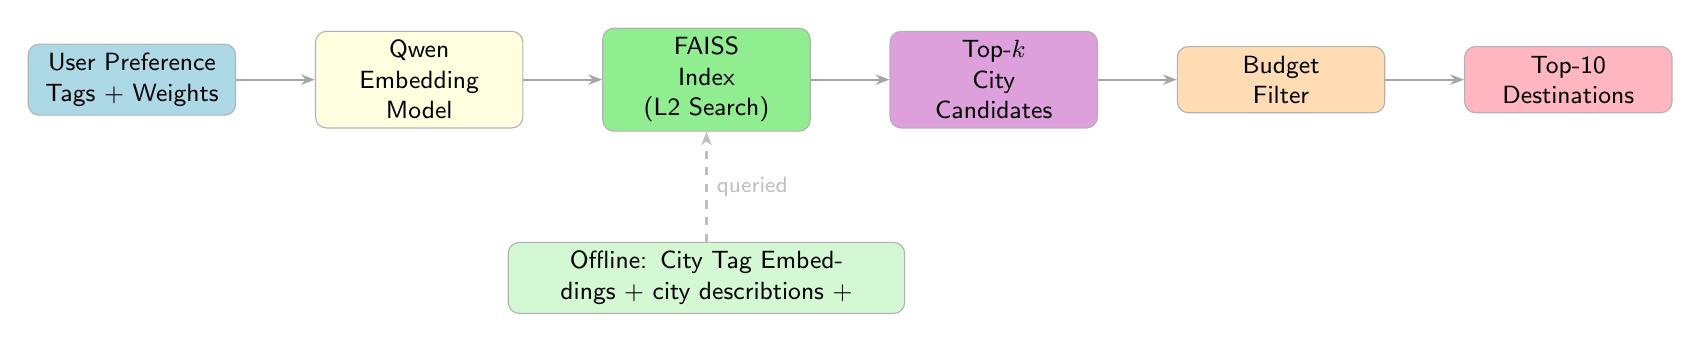
\begin{tikzpicture}[
  node distance=0.5cm and 1.0cm,
  rbox/.style={rectangle, rounded corners=4pt, draw=gray!60, fill=#1,
               minimum width=2.6cm, minimum height=0.8cm,
               text centered, font=\small\sffamily, text width=2.4cm},
  arr/.style={-{Stealth[length=5pt]}, thick, gray!70},
  darr/.style={-{Stealth[length=5pt]}, thick, dashed, gray!50}
]
\node[rbox=lightblue]   (pref)   {User Preference\\Tags + Weights};
\node[rbox=lightyellow, right=1.0cm of pref]  (embed)  {Qwen\\Embedding\\Model};
\node[rbox=lightgreen,  right=1.0cm of embed] (faiss)  {FAISS\\Index\\(L2 Search)};
\node[rbox=lightpurple, right=1.0cm of faiss] (topk)   {Top-$k$\\City\\Candidates};
\node[rbox=lightorange, right=1.0cm of topk]  (filter) {Budget\\Filter};
\node[rbox=lightred,    right=1.0cm of filter](result) {Top-10\\Destinations};
\node[rbox=lightgreen!40, below=1.4cm of faiss, minimum width=5cm, text width=4.8cm]
  (index) {Offline: City Tag Embeddings + city describtions + };
\draw[arr]  (pref)   -- (embed);
\draw[arr]  (embed)  -- (faiss);
\draw[arr]  (faiss)  -- (topk);
\draw[arr]  (topk)   -- (filter);
\draw[arr]  (filter) -- (result);
\draw[darr] (index.north) -- (faiss.south) node[midway,right,font=\footnotesize\sffamily]{queried};
\end{tikzpicture}
}%
\caption{RAG pipeline for destination retrieval: user preferences are embedded at query time and
         searched against the pre-built offline city tag index.}
\label{fig:rag-pipeline}
\end{figure}

\subsection{Vector Databases and Semantic Search}

\textbf{Vector databases} store data as high-dimensional numerical vectors (embeddings). Semantic
similarity is measured by the geometric distance between vectors, enabling retrieval based on meaning
rather than keyword matching. \textbf{FAISS} (Facebook AI Similarity Search) is an open-source
library for efficient similarity search over dense vectors \cite{johnson2019faiss}, widely used for
RAG pipelines and recommendation systems.

\subsection{Workflow Automation and Web Scraping}

\textbf{n8n} is an open-source, node-based workflow automation platform supporting API calls, data
transformations, conditional routing, and LLM invocations within executable visual workflows.
\textbf{Web scraping} is the automated extraction of structured data from web pages; in this project,
it is used to retrieve live hotel and attraction data from Booking.com, with \textbf{Selenium
WebDriver} as a fallback for JavaScript-rendered or bot-protected content.

% ---------------------------------------------------------
\section{Competitor Comparison}
% ---------------------------------------------------------

Table~\ref{tab:competitor-comparison} provides a feature-by-feature comparison of leading travel
planning platforms against TRAVELAI (this project). KimKim is included as a representative of the
high-personalization, low-automation end of the spectrum: it connects travelers with vetted local
human specialists rather than employing an automated AI pipeline.

\begin{table}[htbp]
\centering
\small
\renewcommand{\arraystretch}{1.3}
\begin{tabularx}{\textwidth}{p{3.6cm} *{6}{>{\centering\arraybackslash}X}}
\toprule
\textbf{Feature} & \textbf{TripAdv.} & \textbf{Expedia}
  & \textbf{Layla.ai} & \textbf{TripBuilder}
  & \textbf{KimKim} & \textbf{TRAVELAI} \\
\midrule
Conversational AI      & Partial & Partial & Yes    & No      & No (human chat) & Yes \\
Weather-aware adapt.   & No      & No      & No     & Partial & Manual          & Yes \\
Collaborative planning & Partial & Yes     & Partial & No     & Yes             & Planned \\
Auto itinerary gen.    & Yes     & Partial & Yes    & Yes     & No (human)      & Yes \\
Full trip optimization & No      & No      & Yes    & Yes     & No (human)      & Yes \\
Real-time availability & Yes     & Yes     & Yes    & Yes     & Partial         & Yes \\
Personalized recs.     & Yes     & Yes     & Yes    & Yes     & Yes (human)     & Yes \\
External API integr.   & Partial & Yes     & Yes    & Partial & Unknown         & Yes \\
Direct booking         & Partial & Yes     & Links  & Links   & Yes             & Links \\
RAG-based retrieval    & No      & No      & No     & No      & No              & Yes \\
\bottomrule
\end{tabularx}
\caption{Feature comparison of major travel planning platforms (March 2026).
         KimKim entries marked \emph{human} reflect specialist-driven rather than
         automated capabilities.}
\label{tab:competitor-comparison}
\end{table}

% ---------------------------------------------------------
\section{Competitor Analysis}
% ---------------------------------------------------------

\textbf{Tripadvisor} excels at inspiration and review-driven planning but lacks weather-aware
adaptation and deep budget/time/distance routing. \textbf{Expedia Group} offers strong booking
integration but remains package-oriented rather than multi-agent driven. \textbf{Layla.ai} delivers
excellent chat-based planning but relies on external partners and lacks weather adaptation and group
collaboration. \textbf{TripBuilder.ai} generates fast starting itineraries via forms but requires
manual follow-up for refinements. \textbf{KimKim} takes a different approach entirely: rather than
automating itinerary generation, it matches travelers with vetted local specialists who design
custom trips through a human chat interface. While this delivers high-quality personalization, it
does not scale algorithmically and provides no weather-aware or real-time automated adaptation.

\textbf{TRAVELAI} addresses the automation and intelligence gaps shared by all surveyed platforms
through iterative preference extraction, automatic full itinerary generation, and continuous
optimization across budget, travel time, distance, and weather conditions. Its addition of
RAG-based semantic city retrieval distinguishes it from every surveyed competitor, including the
human-specialist model of KimKim.

\section*{Conclusion}
\addcontentsline{toc}{section}{Conclusion}

This chapter has laid the theoretical groundwork for the project's technical choices and positioned
the system relative to the existing market. The identified gaps --- semantic retrieval, multi-agent
orchestration, and weather-aware planning --- motivate the architecture described in the
following chapters.
% =========================================================
%  CHAPTER 3 — DATA COLLECTION
% =========================================================
\chapter{Data Collection}

\section*{Introduction}
\addcontentsline{toc}{section}{Introduction}

This chapter describes the two main data categories underpinning the travel planner: \textbf{static
data}, collected and processed offline in advance, and \textbf{dynamic data}, fetched in real time
during each planning session. Together they provide both broad destination knowledge and up-to-date
situational awareness.

% ---------------------------------------------------------
\section{Static Data}
% ---------------------------------------------------------

Static data provides the stable semantic foundation for destination discovery, drawn from three
main sources.

\textbf{POI Dataset.} Derived from \texttt{wikivoyage-listing.csv}, this file contains structured
listings of attractions, restaurants, hotels, and activities. A preprocessing phase removed
incomplete or duplicate entries, standardized formats, and filtered for tourism-relevant listings.

\textbf{Wikivoyage Destination Descriptions.} Rich textual descriptions of cities providing
contextual information about history, atmosphere, cultural aspects, and available activities. Only
cities with sufficiently detailed descriptions were retained.

\textbf{City Dataset and Tag Generation.} Starting from \texttt{worldcities.csv}, cities above a
minimum population threshold were selected (no subcountry/regional substitution is applied) and then
filtered to retain only those with a Wikivoyage description, yielding roughly 1,500 cities. Each
retained city was annotated with descriptive tourism tags using a language model to facilitate
semantic comparison.

% ---------------------------------------------------------
\section{Static Data Preprocessing Pipeline}
\label{sec:preprocessing}
% ---------------------------------------------------------

A multi-stage offline preprocessing pipeline transforms the raw static datasets into two primary
artefacts: a structured \textbf{POI dataset} and a \textbf{FAISS vector index} for fast semantic
city search. Figure~\ref{fig:preprocessing} illustrates the five sequential stages; full technical
details are provided in Appendix~\ref{app:preprocessing}.

\begin{figure}[H]
\centering
\resizebox{0.85\linewidth}{!}{%
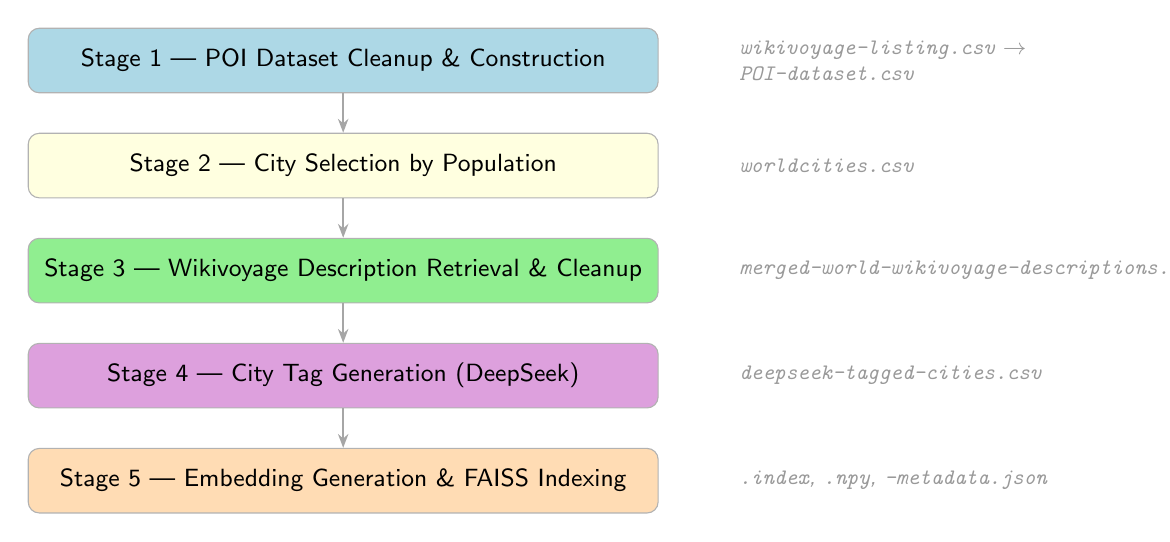
\begin{tikzpicture}[
  node distance = 0.5cm,
  stagebox/.style = {rectangle, rounded corners=4pt, draw=gray!60,
                     minimum width=8cm, minimum height=0.82cm,
                     text centered, font=\small\sffamily},
  ann/.style = {font=\footnotesize\sffamily\itshape, text=gray!80, text width=5cm},
  arr/.style = {-{Stealth[length=5pt]}, thick, gray!70}
]
\node[stagebox, fill=lightblue]   (s1) {Stage 1 --- POI Dataset Cleanup \& Construction};
\node[stagebox, fill=lightyellow, below=of s1] (s2) {Stage 2 --- City Selection by Population};
\node[stagebox, fill=lightgreen,  below=of s2] (s3) {Stage 3 --- Wikivoyage Description Retrieval \& Cleanup};
\node[stagebox, fill=lightpurple, below=of s3] (s4) {Stage 4 --- City Tag Generation (DeepSeek)};
\node[stagebox, fill=lightorange, below=of s4] (s5) {Stage 5 --- Embedding Generation \& FAISS Indexing};
\draw[arr] (s1) -- (s2);
\draw[arr] (s2) -- (s3);
\draw[arr] (s3) -- (s4);
\draw[arr] (s4) -- (s5);
\node[ann, right=0.9cm of s1] {\texttt{wikivoyage-listing.csv} $\rightarrow$ \texttt{POI-dataset.csv}};
\node[ann, right=0.9cm of s2] {\texttt{worldcities.csv}};
\node[ann, right=0.9cm of s3] {\texttt{merged-world-wikivoyage-descriptions.csv}};
\node[ann, right=0.9cm of s4] {\texttt{deepseek-tagged-cities.csv}};
\node[ann, right=0.9cm of s5] {\texttt{.index}, \texttt{.npy}, \texttt{-metadata.json}};
\end{tikzpicture}
}%
\caption{Five-stage offline data preprocessing pipeline, from raw Wikivoyage listings to a FAISS
         vector index.}
\label{fig:preprocessing}
\end{figure}

\begin{table}[htbp]
\centering
\small
\renewcommand{\arraystretch}{1.3}
\begin{tabularx}{\textwidth}{
    >{\centering\arraybackslash}p{0.4cm}
    >{\raggedright\arraybackslash}p{3.5cm}
    >{\raggedright\arraybackslash}p{3.8cm}
    >{\raggedright\arraybackslash}X}
\toprule
\textbf{\#} & \textbf{Stage} & \textbf{Input} & \textbf{Output} \\
\midrule
1 & POI Cleanup \& Construction & \texttt{wikivoyage-listing.csv}, \texttt{worldcities.csv} & \texttt{POI-dataset.csv} \\
2 & City Selection by Population & \texttt{worldcities.csv} & Selected city list \\
3 & Description Retrieval \& Cleanup & Selected cities + Wikivoyage descriptions & \texttt{merged-world-wikivoyage-descriptions.csv} \\
4 & Tag Generation (DeepSeek) & City descriptions + DeepSeek API & \texttt{deepseek-tagged-cities.csv} \\
5 & Embeddings \& FAISS     & Tagged cities + Qwen model & \texttt{.index}, \texttt{.npy}, \texttt{-metadata.json} \\
\bottomrule
\end{tabularx}
\caption{Summary of the five preprocessing pipeline stages, their inputs, and output artefacts.}
\label{tab:preprocessing-summary}
\end{table}

\paragraph{Stage 1.} Cleans and constructs the POI dataset: the raw Wikivoyage listings are filtered
to retain only cities present in the WorldCities reference, incomplete and duplicate rows are removed,
and the schema is normalized to five columns (city, country, type, title, description) before the
listings are assembled into \texttt{POI-dataset.csv}.

\paragraph{Stage 2.} Selects candidate cities from the WorldCities reference, keeping those above a
minimum population threshold. Unlike the earlier design, \emph{no} subcountry/regional substitution is
performed; cities are carried through under their own names.

\paragraph{Stage 3.} Retrieves and merges the Wikivoyage prose descriptions for the selected cities
into a single canonical file, applying Unicode normalization (diacritic removal, case folding,
apostrophe standardization) and deduplication, and keeping only cities that have a non-empty
description.

\paragraph{Stage 4.} Annotates each of the approximately 1,500 described cities with descriptive
tourism tags using DeepSeek. The city description is first cleaned and truncated, then tags are drawn
from a fixed vocabulary of 22 descriptors (see Appendix~\ref{app:tag-vocabulary}) with floating-point
weights in $[0.0, 1.0]$.

\paragraph{Stage 5.} Computes 1024-dimensional city embeddings using the Qwen model via a weighted
mean over tag vectors. All city vectors are assembled into a FAISS \texttt{IndexFlatL2} index.
Two additional indices (POI chunk and city description) are also built for attraction-level and
narrative-level retrieval.

% ---------------------------------------------------------
\section{Dynamic Data}
% ---------------------------------------------------------

The system relies on \textbf{dynamic data} fetched in real time during each planning session to
ensure every itinerary reflects current conditions at the moment of planning. Three external
providers are integrated.

\textbf{Booking.com Scraper.} For each candidate destination, the scraper queries Booking.com for
live hotel availability, nightly prices, user review scores, and nearby points of interest. When
anti-bot challenges are detected, a Selenium WebDriver fallback is used.

\textbf{SerpAPI (Google Flights).} For each candidate destination, the Planner agent constructs a
flight query returning available options with airline, duration, stops, real-time ticket prices, and
booking links.

\textbf{Open-Meteo API.} A free, open-source weather forecast API providing high-resolution
multi-day forecasts by geographic coordinates. The Planner agent uses day-by-day temperature,
precipitation, and weather condition data to align outdoor activities with favorable conditions.

Figure~\ref{fig:dynamic-pipeline} shows how these three providers are queried concurrently once
the top-3 candidate cities are identified, and how results are merged before the Planner agent.

\begin{figure}[H]
\centering
\resizebox{0.9\linewidth}{!}{%
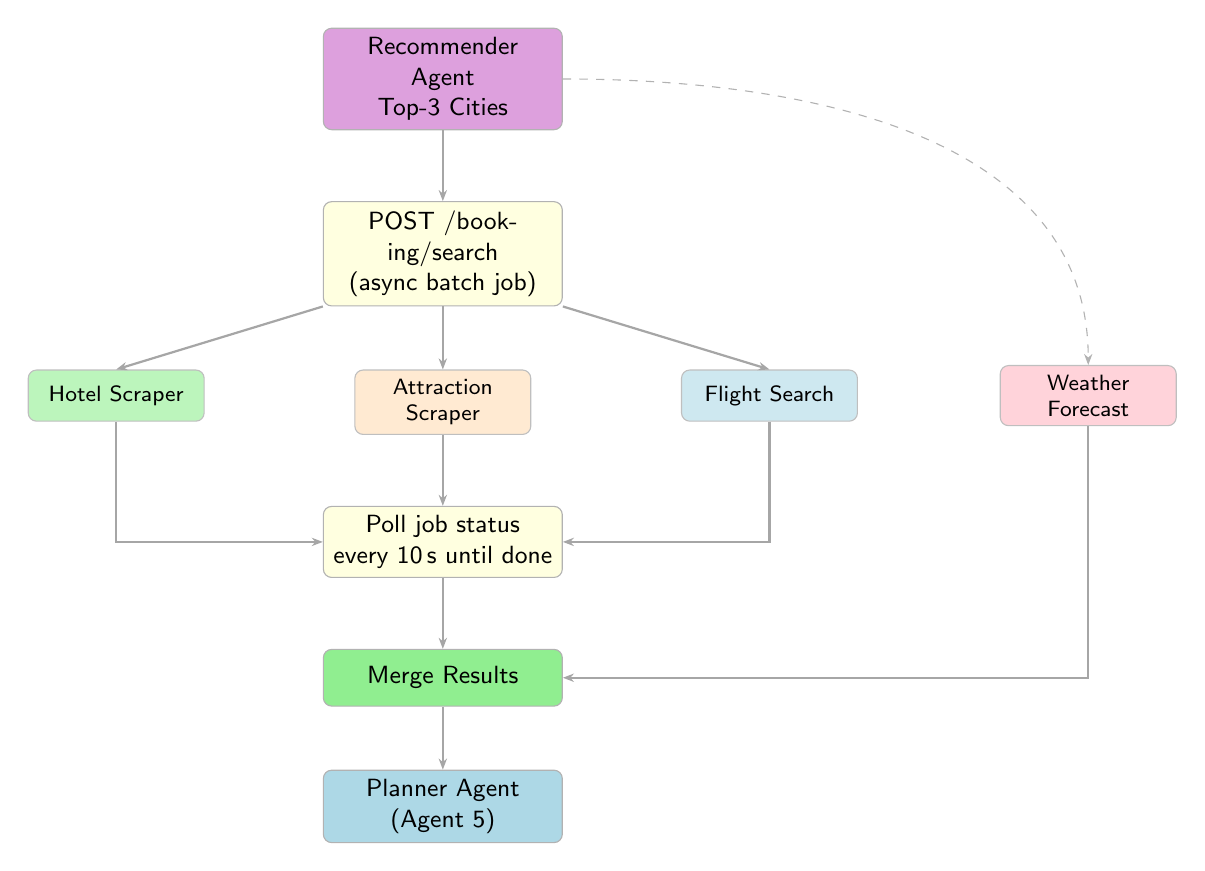
\begin{tikzpicture}[
  node distance=0.5cm and 0.8cm,
  pbox/.style={rectangle, rounded corners=3pt, draw=gray!60, fill=#1,
               minimum width=3.0cm, minimum height=0.72cm,
               text centered, font=\small\sffamily, text width=2.8cm},
  sbox/.style={rectangle, rounded corners=3pt, draw=gray!50, fill=#1,
               minimum width=2.2cm, minimum height=0.65cm,
               text centered, font=\footnotesize\sffamily, text width=2.0cm},
  arr/.style={-{Stealth[length=4pt]}, thick, gray!70},
  darr/.style={-{Stealth[length=4pt]}, dashed, gray!60}
]
\node[pbox=lightpurple] (rec) {Recommender Agent\\Top-3 Cities};
\node[pbox=lightyellow, below=0.9cm of rec] (post) {POST /booking/search\\(async batch job)};
\draw[arr] (rec) -- (post);

\node[sbox=lightgreen!60,  below left=0.8cm and 1.5cm of post]  (hotel)  {Hotel Scraper};
\node[sbox=lightorange!60, below=0.8cm of post]                  (attr)   {Attraction Scraper};
\node[sbox=lightblue!60,   below right=0.8cm and 1.5cm of post] (flight) {Flight Search};
\node[sbox=lightred!60,    right=1.8cm of flight]               (wx)     {Weather Forecast};

\draw[arr] (post.south west) -- (hotel.north);
\draw[arr] (post.south)      -- (attr.north);
\draw[arr] (post.south east) -- (flight.north);
\draw[darr] (rec.east) to[out=0,in=90] (wx.north);

\node[pbox=lightyellow, below=0.9cm of attr] (poll) {Poll job status\\every 10\,s until done};
\draw[arr] (hotel.south)  |- (poll.west);
\draw[arr] (attr.south)   -- (poll.north);
\draw[arr] (flight.south) |- (poll.east);

\node[pbox=lightgreen, below=0.9cm of poll] (merge) {Merge Results};
\draw[arr] (poll)     -- (merge);
\draw[arr] (wx.south) |- (merge.east);

\node[pbox=lightblue, below=0.8cm of merge] (plan) {Planner Agent (Agent 5)};
\draw[arr] (merge) -- (plan);
\end{tikzpicture}
}%
\caption{Dynamic data pipeline: hotels, attractions, flights, and weather are fetched concurrently
         via an asynchronous batch job for the top-3 cities, then merged before itinerary assembly.}
\label{fig:dynamic-pipeline}
\end{figure}

\begin{table}[htbp]
\centering
\small
\renewcommand{\arraystretch}{1.3}
\begin{tabularx}{\textwidth}{
    >{\raggedright\arraybackslash}p{2.8cm}
    >{\raggedright\arraybackslash}p{3.0cm}
    >{\raggedright\arraybackslash}X
    >{\raggedright\arraybackslash}p{3.2cm}}
\toprule
\textbf{Source} & \textbf{Provider} & \textbf{Data Collected} & \textbf{Used By} \\
\midrule
Hotel \& POI Data
  & Booking.com Scraper
  & Hotel pricing, availability, reviews, nearby POIs
  & Recommender, Planner \\
Flight Data
  & SerpAPI (Google Flights)
  & Flight options, prices, durations, booking links
  & Planner Agent \\
Weather Forecasts
  & Open-Meteo API
  & Daily temperature, precipitation, wind, conditions
  & Planner Agent \\
\bottomrule
\end{tabularx}
\caption{Dynamic data sources, the data they provide, and the agents that consume them.}
\label{tab:dynamic-data}
\end{table}

\section*{Conclusion}
\addcontentsline{toc}{section}{Conclusion}

This chapter has described the two data layers underpinning the system. The static layer provides a
stable semantic knowledge base covering approximately 1,500 well-documented tourist destinations.
The dynamic layer grounds every generated itinerary in real-world conditions at the time of
planning.

% =========================================================
%  CHAPTER 4 — SYSTEM ARCHITECTURE
% =========================================================
\chapter{System Architecture}

\section*{Introduction}
\addcontentsline{toc}{section}{Introduction}

This chapter presents the overall architecture of the AI-Powered Multi-Agent Travel Planner,
covering the orchestration layer, the four specialized AI agents, the session state machine, the
end-to-end pipeline, and the deployment topology.

% ---------------------------------------------------------
\section{Overview}
% ---------------------------------------------------------

The system is built on an \textbf{orchestrator-centric multi-agent architecture} implemented using
n8n. A central orchestrator maintains session state, routes control flow between specialized AI
agents, and coordinates external data integration. The architecture is composed of five layers:
the \textbf{User Layer} (HTTP webhook entry), the \textbf{Orchestrator Layer} (session state and
routing), the \textbf{AI Agents Layer} (four LLM-powered agents), the \textbf{External APIs Layer}
(hotels, flights, weather), and the \textbf{Static Data Layer} (POIs, city tags, vector index).
Figure~\ref{fig:architecture} illustrates the complete data flow.

\begin{figure}[H]
\centering
\resizebox{\linewidth}{!}{%
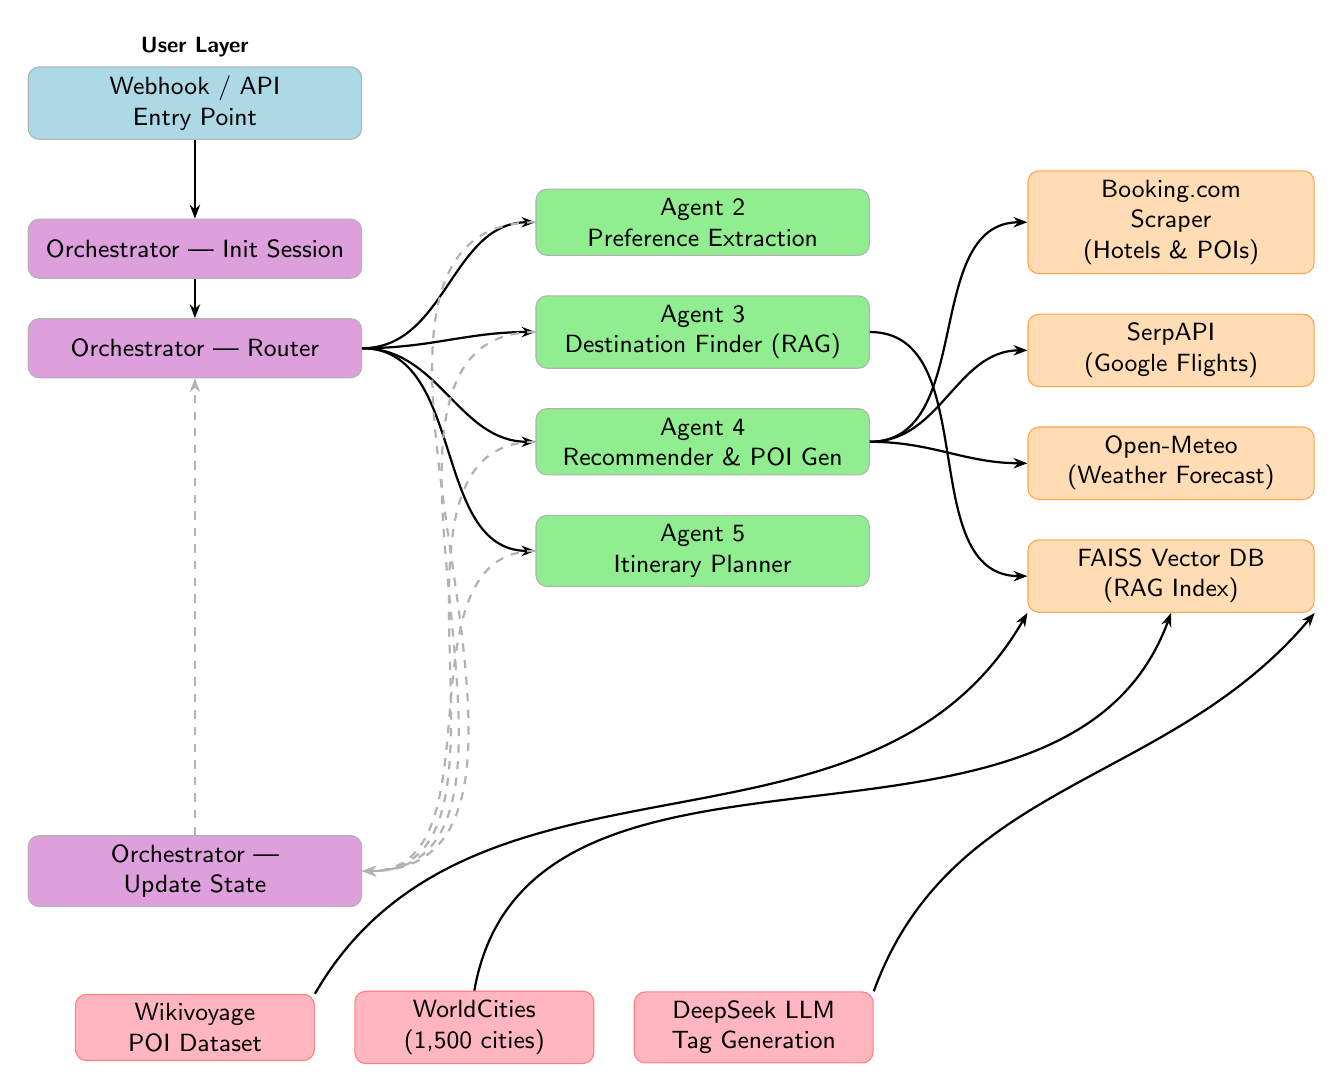
\begin{tikzpicture}[
  node distance = 0.45cm and 1.5cm,
  every node/.style = {font=\small\sffamily},
  box/.style    = {rectangle, rounded corners=4pt, draw=gray!60,
                   fill=#1, minimum width=4.2cm, minimum height=0.75cm,
                   text centered, text width=4cm},
  extbox/.style = {rectangle, rounded corners=4pt, draw=orange!70,
                   fill=lightorange, minimum width=3.6cm, minimum height=0.75cm,
                   text centered, text width=3.4cm},
  staticbox/.style={rectangle, rounded corners=4pt, draw=red!50,
                   fill=lightred, minimum width=3cm, minimum height=0.75cm,
                   text centered, text width=2.8cm},
  arr/.style    = {-{Stealth[length=5pt]}, thick},
  darr/.style   = {-{Stealth[length=5pt]}, thick, dashed, gray!60}
]
\node[box=lightblue, label={[font=\footnotesize\sffamily]above:{\textbf{User Layer}}}]
  (webhook) {Webhook / API\\Entry Point};
\node[box=lightpurple, below=1.0cm of webhook]
  (orch_init) {Orchestrator --- Init Session};
\node[box=lightpurple, below=0.5cm of orch_init]
  (orch_router) {Orchestrator --- Router};
\node[box=lightpurple, below=5.8cm of orch_router]
  (orch_update) {Orchestrator --- Update State};

\node[box=lightgreen, right=2.2cm of orch_router, yshift=1.6cm]
  (a2) {Agent 2\\Preference Extraction};
\node[box=lightgreen, below=0.5cm of a2]
  (a3) {Agent 3\\Destination Finder (RAG)};
\node[box=lightgreen, below=0.5cm of a3]
  (a4) {Agent 4\\Recommender \& POI Gen};
\node[box=lightgreen, below=0.5cm of a4]
  (a5) {Agent 5\\Itinerary Planner};

\node[extbox, right=2.0cm of a2]
  (booking) {Booking.com\\Scraper\\(Hotels \& POIs)};
\node[extbox, below=0.5cm of booking]
  (serp)    {SerpAPI\\(Google Flights)};
\node[extbox, below=0.5cm of serp]
  (weather) {Open-Meteo\\(Weather Forecast)};
\node[extbox, below=0.5cm of weather]
  (faiss)   {FAISS Vector DB\\(RAG Index)};

\node[staticbox, below=1.1cm of orch_update]
  (wiki)  {Wikivoyage\\POI Dataset};
\node[staticbox, right=0.5cm of wiki]
  (wc)    {WorldCities\\(1{,}500 cities)};
\node[staticbox, right=0.5cm of wc]
  (groq)  {DeepSeek LLM\\Tag Generation};

\draw[arr] (webhook)     -- (orch_init);
\draw[arr] (orch_init)   -- (orch_router);
\draw[arr] (orch_router.east) to[out=0,in=180]  (a2.west);
\draw[arr] (orch_router.east) to[out=0,in=180]  (a3.west);
\draw[arr] (orch_router.east) to[out=0,in=180]  (a4.west);
\draw[arr] (orch_router.east) to[out=0,in=180]  (a5.west);
\draw[darr] (a2.west) to[out=180,in=0] (orch_update.east);
\draw[darr] (a3.west) to[out=180,in=0] (orch_update.east);
\draw[darr] (a4.west) to[out=180,in=0] (orch_update.east);
\draw[darr] (a5.west) to[out=180,in=0] (orch_update.east);
\draw[darr] (orch_update.north) -- (orch_router.south);
\draw[arr] (a4.east) to[out=0,in=180] (booking.west);
\draw[arr] (a4.east) to[out=0,in=180] (serp.west);
\draw[arr] (a4.east) to[out=0,in=180] (weather.west);
\draw[arr] (a3.east) to[out=0,in=180] (faiss.west);
\draw[arr] (wiki.north east) to[out=60,in=240]  (faiss.south west);
\draw[arr] (wc.north)        to[out=80,in=250]  (faiss.south);
\draw[arr] (groq.north east) to[out=70,in=230]  (faiss.south east);
\end{tikzpicture}
}%
\caption{Overall system architecture showing the five layers and data flows between them.}
\label{fig:architecture}
\end{figure}

% ---------------------------------------------------------
\section{Use Case Diagram}
% ---------------------------------------------------------
Figure~\ref{fig:usecase} presents the system's use case model from the perspective of the
authenticated traveler --- the sole external actor.

\begin{figure}[H]
\centering
\resizebox{0.85\linewidth}{!}{%
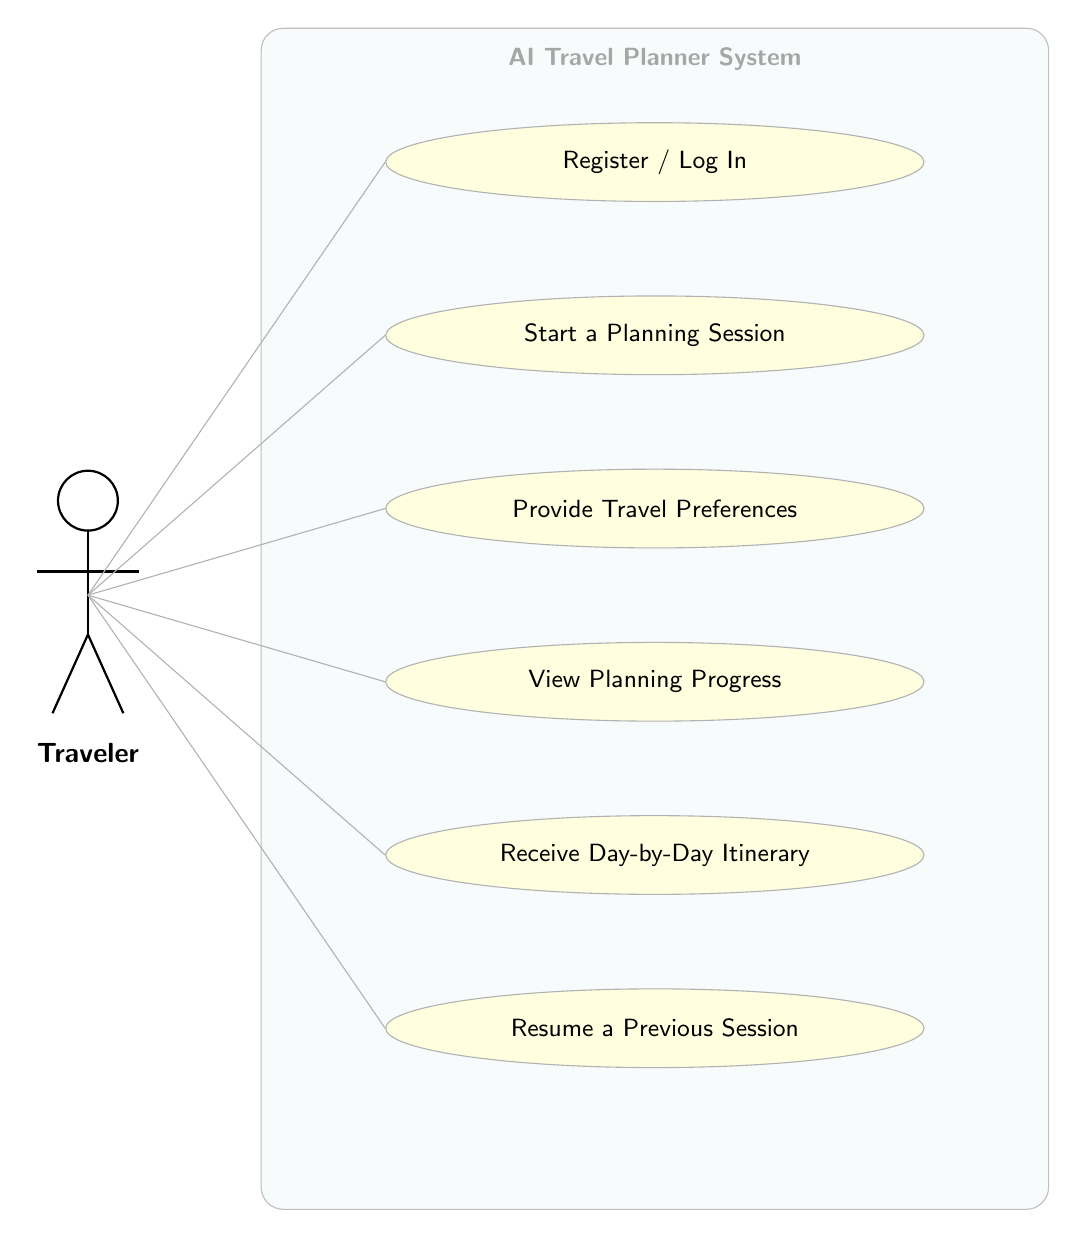
\begin{tikzpicture}[
  every node/.style={font=\small\sffamily},
  uc/.style={ellipse, draw=gray!60, fill=lightyellow, minimum width=5.0cm,
             minimum height=1.0cm, text centered, text width=4.6cm}
]

% System boundary
\draw[draw=gray!50, fill=lightblue!10, rounded corners=8pt]
  (1.0, 0.5) rectangle (11.0,-14.5);
\node[font=\small\bfseries\sffamily, text=gray!70] at (6, 0.1)
  {AI Travel Planner System};

% Use case ellipses — 2.2cm gap between each
\node[uc] (uc1) at (6, -1.2) {Register / Log In};
\node[uc] (uc2) at (6, -3.4) {Start a Planning Session};
\node[uc] (uc3) at (6, -5.6) {Provide Travel Preferences};
\node[uc] (uc4) at (6, -7.8) {View Planning Progress};
\node[uc] (uc5) at (6,-10.0) {Receive Day-by-Day Itinerary};
\node[uc] (uc6) at (6,-12.2) {Resume a Previous Session};

% Actor stick figure centered vertically on the use cases
\draw[thick] (-1.2,-5.5) circle (0.38cm);          % head
\draw[thick] (-1.2,-5.88) -- (-1.2,-7.2);          % body
\draw[thick] (-1.85,-6.4) -- (-0.55,-6.4);         % arms
\draw[thick] (-1.2,-7.2) -- (-1.65,-8.2);          % left leg
\draw[thick] (-1.2,-7.2) -- (-0.75,-8.2);          % right leg
\node[font=\normalsize\sffamily\bfseries] at (-1.2,-8.7) {Traveler};

% Association lines from actor torso centre to each use case
\foreach \uc in {uc1,uc2,uc3,uc4,uc5,uc6}{
  \draw[gray!60] (-1.2,-6.7) -- (\uc.west);
}

\end{tikzpicture}
}%
\caption{Use case diagram of the AI-Powered Multi-Agent Travel Planner. The Traveler is the sole
         external actor; all planning logic is internal to the system.}
\label{fig:usecase}
\end{figure}


% ---------------------------------------------------------
\section{Session State Machine}
% ---------------------------------------------------------

The \texttt{tripContext} object maintained by the orchestrator follows a well-defined state machine.
Figure~\ref{fig:statemachine} shows the states and transitions driven by agent outcomes.

\begin{figure}[H]
\centering
\resizebox{0.75\linewidth}{!}{%
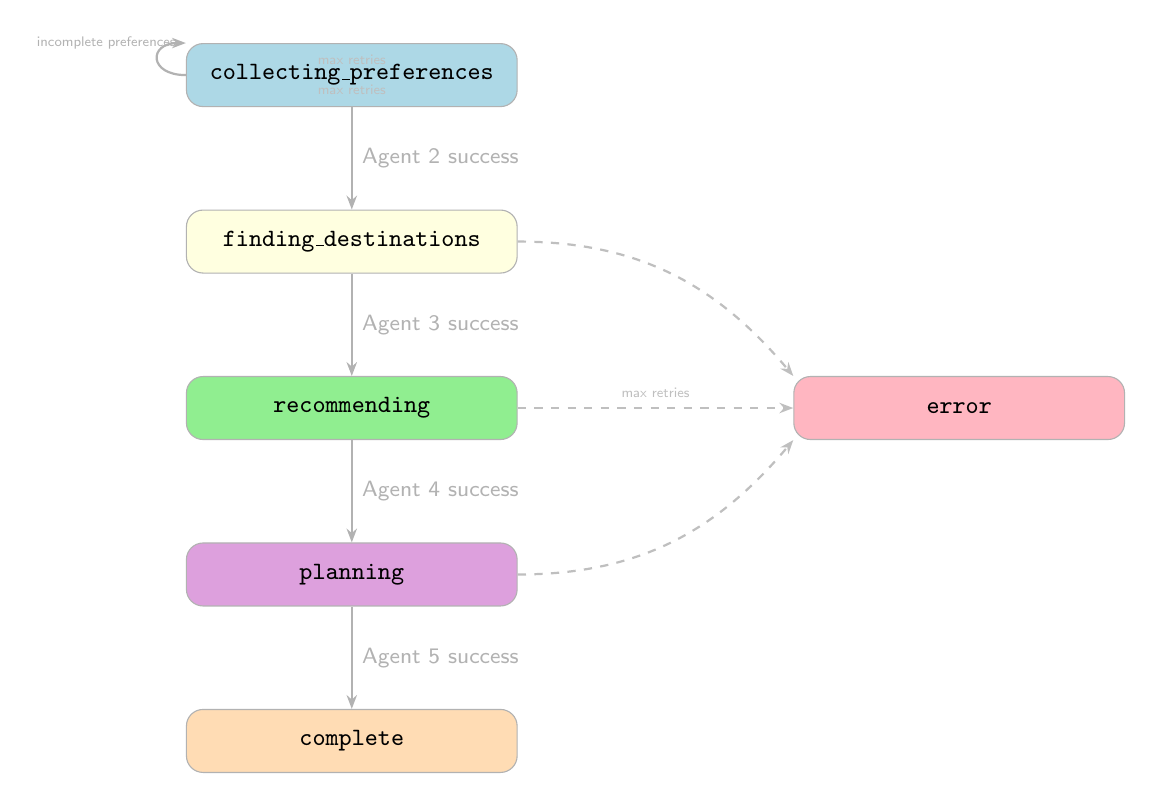
\begin{tikzpicture}[
  every node/.style={font=\small\sffamily},
  state/.style={rectangle, rounded corners=6pt, draw=gray!60, fill=#1,
                minimum width=4.2cm, minimum height=0.8cm, text centered},
  arr/.style={-{Stealth[length=5pt]}, thick, gray!60},
  darr/.style={-{Stealth[length=5pt]}, thick, dashed, gray!50},
  node distance=1.3cm
]
\node[state=lightblue]   (s1) {\texttt{collecting\_preferences}};
\node[state=lightyellow, below=of s1] (s2) {\texttt{finding\_destinations}};
\node[state=lightgreen,  below=of s2] (s3) {\texttt{recommending}};
\node[state=lightpurple, below=of s3] (s4) {\texttt{planning}};
\node[state=lightorange, below=of s4] (s5) {\texttt{complete}};
\node[state=lightred,    right=3.5cm of s3] (err) {\texttt{error}};

\draw[arr] (s1) -- (s2) node[midway, right, font=\footnotesize\sffamily]{Agent 2 success};
\draw[arr] (s2) -- (s3) node[midway, right, font=\footnotesize\sffamily]{Agent 3 success};
\draw[arr] (s3) -- (s4) node[midway, right, font=\footnotesize\sffamily]{Agent 4 success};
\draw[arr] (s4) -- (s5) node[midway, right, font=\footnotesize\sffamily]{Agent 5 success};

\draw[darr] (s2.east) to[out=0,in=130] (err.north west)
  node[near start, above, font=\tiny\sffamily]{max retries};
\draw[darr] (s3.east) -- (err.west)
  node[midway, above, font=\tiny\sffamily]{max retries};
\draw[darr] (s4.east) to[out=0,in=230] (err.south west)
  node[near start, below, font=\tiny\sffamily]{max retries};
\draw[arr] (s1.west) to[out=180,in=180, looseness=3] (s1.north west)
  node[left, font=\tiny\sffamily]{incomplete preferences};
\end{tikzpicture}
}%
\caption{Session state machine: \texttt{tripContext.status} transitions through five sequential
         stages. Failure after maximum retries leads to the \texttt{error} state; incomplete
         preferences loop Agent~2 until all fields are collected.}
\label{fig:statemachine}
\end{figure}

% ---------------------------------------------------------
\section{Orchestrator and AI Agents Layer}
% ---------------------------------------------------------

\paragraph{Session Initialization.}
When a new request arrives, the orchestrator creates or restores a \texttt{tripContext} object that
tracks extracted preferences, destination candidates, recommended cities, agent results, conversation
history, and the current pipeline stage. Sessions are identified by unique UUIDs stored in n8n's
static workflow data. The \texttt{status} field transitions in a strict one-way sequence:
$\texttt{collecting\_preferences} \to \texttt{finding\_destinations} \to \texttt{recommending}
\to \texttt{planning} \to \texttt{complete}$.

\paragraph{Routing.}
At each step the orchestrator evaluates the \texttt{next\_action} field and routes to the
appropriate agent: Agent~2 (preference extraction), Agent~3 (destination finder), Agent~4
(recommender), Agent~5 (planner), or a direct webhook response.

All agents are powered by \textbf{DeepSeek} via an OpenAI-compatible API endpoint, each equipped
with a window-based memory buffer (last 10 messages) keyed to the session ID.

\textbf{Agent 2 — Preference Extraction:} engages the user in a one-question-at-a-time interview
to collect departure date, trip duration, departure location, traveler count, budget, travel style,
and preference tags from a 22-descriptor vocabulary with relevance weights. When complete, it emits
a structured JSON block delimited by \texttt{---PREFERENCES\_COMPLETE---}.

\textbf{Agent 3 — Destination Finder:} constructs a weighted tag query and submits it to the FAISS
city matching microservice, returning the top candidate cities ranked by semantic similarity and
budget compatibility.

\textbf{Agent 4 — Recommender and POI Generator:} selects the best 5 from the top 10 candidate
cities, generates 15 richly described Points of Interest per city, and triggers parallel data
requests to Booking.com, SerpAPI, and Open-Meteo for the top 3 cities.

\textbf{Agent 5 — Itinerary Planner:} receives the enriched data for the top 3 cities and generates
a complete day-by-day itinerary with morning/afternoon/evening activity blocks, estimated costs,
weather-aware scheduling, hotel recommendation, packing suggestions, and a full cost breakdown.

% ---------------------------------------------------------
\section{End-to-End Pipeline Flow}
% ---------------------------------------------------------

\begin{figure}[H]
\centering
\resizebox{0.75\linewidth}{!}{%
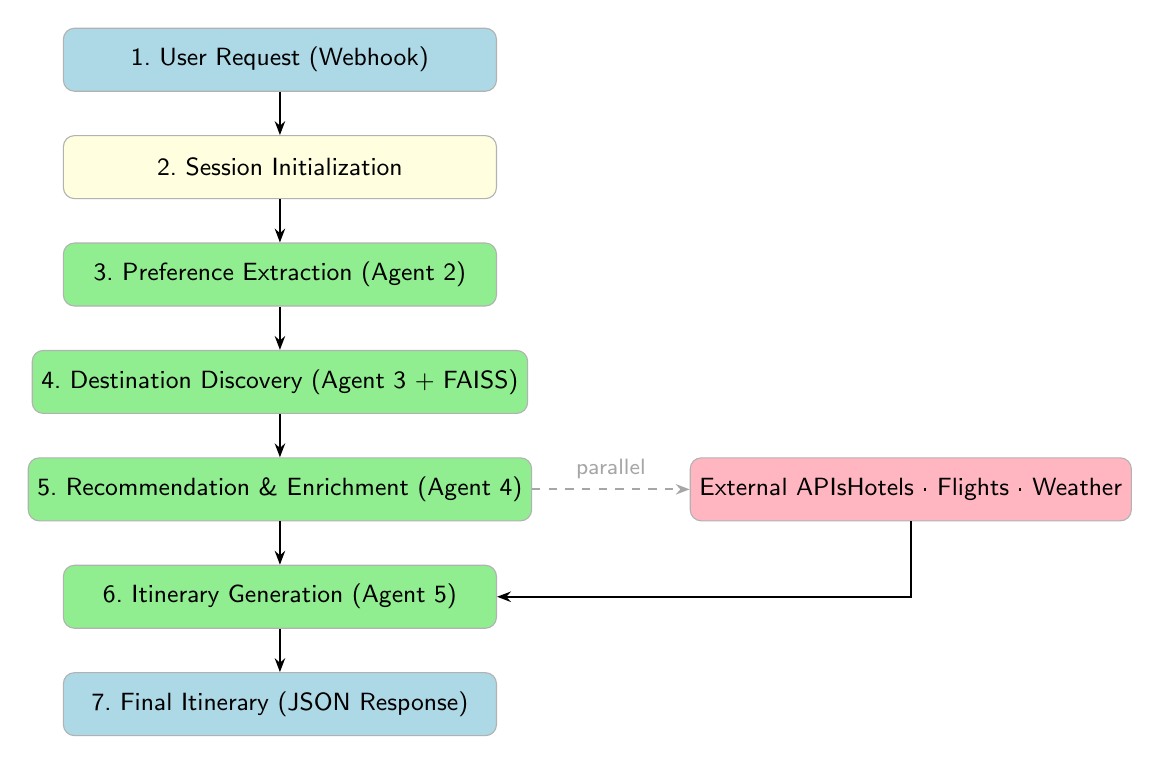
\begin{tikzpicture}[
  node distance = 0.55cm,
  box/.style    = {rectangle, rounded corners=4pt,
                   minimum width=5.5cm, minimum height=0.8cm,
                   text centered, draw=gray!60, font=\small\sffamily},
  arr/.style    = {-{Stealth[length=5pt]}, thick},
  darr/.style   = {-{Stealth[length=5pt]}, thick, dashed, gray!70}
]
\node[box, fill=lightblue]   (req)   {1.\ User Request (Webhook)};
\node[box, fill=lightyellow, below=of req]  (init)  {2.\ Session Initialization};
\node[box, fill=lightgreen,  below=of init] (pref)  {3.\ Preference Extraction (Agent 2)};
\node[box, fill=lightgreen,  below=of pref] (dest)  {4.\ Destination Discovery (Agent 3 + FAISS)};
\node[box, fill=lightgreen,  below=of dest] (rec)   {5.\ Recommendation \& Enrichment (Agent 4)};
\node[box, fill=lightred,    right=2.0cm of rec]
                                             (ext)   {External APIs\\Hotels · Flights · Weather};
\node[box, fill=lightgreen,  below=of rec]  (plan)  {6.\ Itinerary Generation (Agent 5)};
\node[box, fill=lightblue,   below=of plan] (out)   {7.\ Final Itinerary (JSON Response)};

\draw[arr]  (req)  -- (init);
\draw[arr]  (init) -- (pref);
\draw[arr]  (pref) -- (dest);
\draw[arr]  (dest) -- (rec);
\draw[arr]  (rec)  -- (plan);
\draw[arr]  (plan) -- (out);
\draw[darr] (rec)  -- (ext)  node[midway, above, font=\footnotesize\sffamily]{parallel};
\draw[arr]  (ext)  |- (plan);
\end{tikzpicture}
}%
\caption{End-to-end pipeline flow. External API calls at Stage~5 are triggered in parallel to
         minimize latency.}
\label{fig:pipeline}
\end{figure}

The full pipeline can take several minutes, so the system uses an \textbf{asynchronous ACK--poll}
pattern: the webhook immediately returns an acknowledgement and a session ID; the pipeline continues
executing asynchronously; the client waits 30~seconds then polls a status endpoint every second, up
to a maximum of 20~minutes.

\paragraph{Performance Profile.}
The system exhibits two distinct profiles. The \textbf{conversational phase} ($\sim$20--45\,s per
turn) depends primarily on DeepSeek API latency. The \textbf{planning phase} ($\sim$10--15\,min
total) is driven by two compounding factors: sequential Booking.com scraping with deliberate
anti-bot delays (2--5\,s per request across 3 cities $\times$ 2 scrapers) and large-prompt LLM
inference (30--90\,s per agent call). Three remediation paths exist: parallel scraping, professional
scraping APIs (e.g., ScraperAPI), and a higher-capacity LLM — each evaluated in Chapter~6.

% ---------------------------------------------------------
\section{Deployment Architecture}
% ---------------------------------------------------------

Figure~\ref{fig:deployment} shows the physical deployment topology of the system.

\begin{figure}[H]
\centering
\resizebox{\linewidth}{!}{%
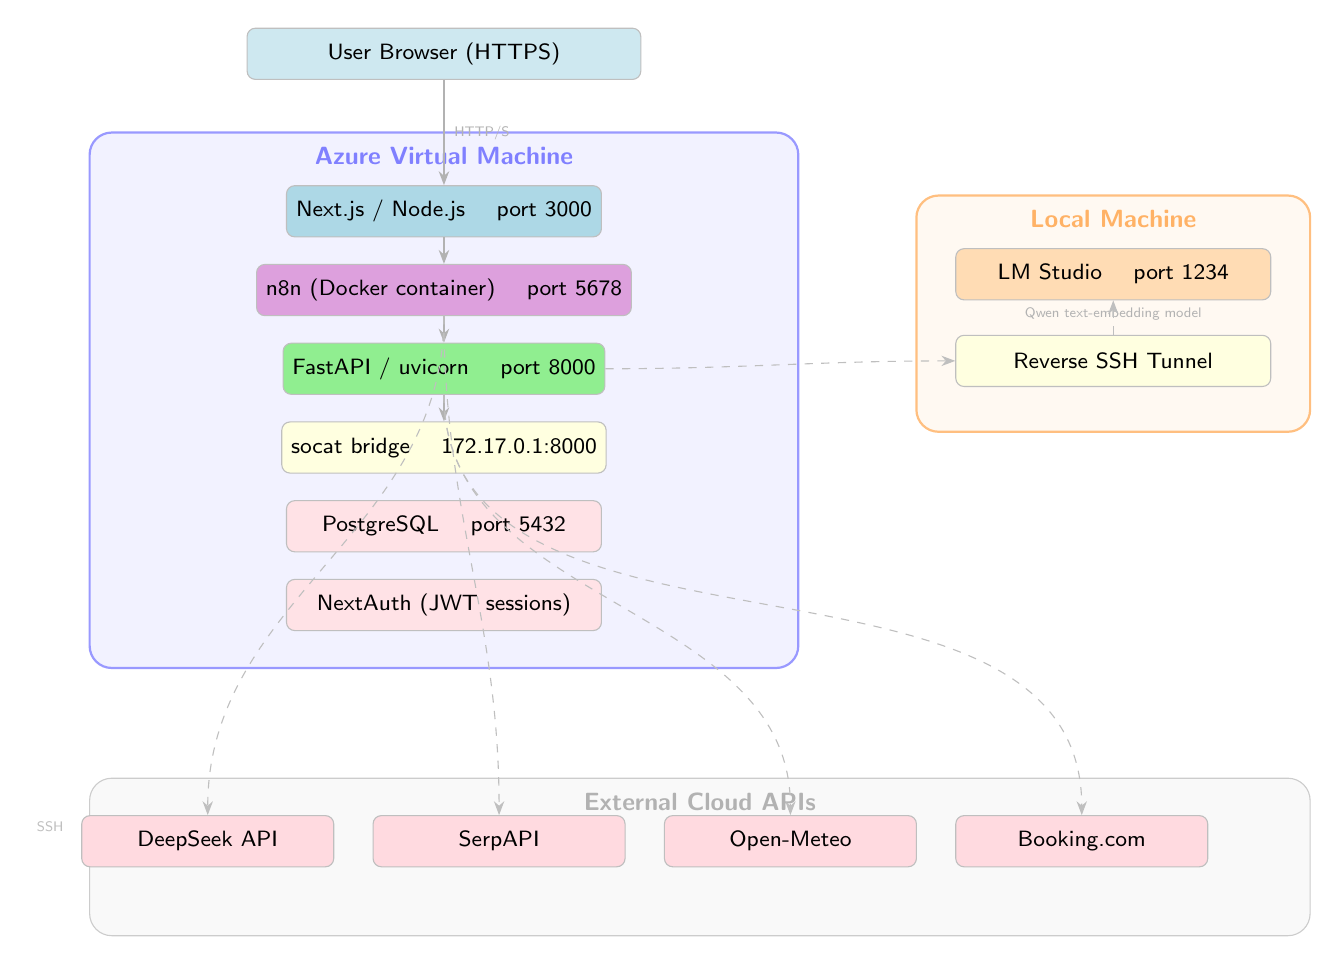
\begin{tikzpicture}[
  every node/.style={font=\small\sffamily},
  svc/.style={rectangle, rounded corners=3pt, draw=gray!50, fill=#1,
              minimum width=4.0cm, minimum height=0.65cm,
              text centered, font=\footnotesize\sffamily},
  arr/.style={-{Stealth[length=5pt]}, thick, gray!60},
  darr/.style={-{Stealth[length=5pt]}, dashed, gray!50}
]
\node[svc=lightblue!60, minimum width=5cm] (browser) at (5,10)
  {User Browser (HTTPS)};

\draw[draw=blue!40, fill=blue!5, rounded corners=8pt, thick]
  (0.5,2.2) rectangle (9.5,9.0);
\node[font=\small\bfseries\sffamily, text=blue!50] at (5,8.7) {Azure Virtual Machine};

\node[svc=lightblue]   (nextjs)  at (5,8.0) {Next.js / Node.js \quad port 3000};
\node[svc=lightpurple] (n8ndock) at (5,7.0) {n8n (Docker container) \quad port 5678};
\node[svc=lightgreen]  (fastapi) at (5,6.0) {FastAPI / uvicorn \quad port 8000};
\node[svc=lightyellow] (socat)   at (5,5.0) {socat bridge \quad 172.17.0.1:8000};
\node[svc=lightred!40] (pg)      at (5,4.0) {PostgreSQL \quad port 5432};
\node[svc=lightred!40] (nauth)   at (5,3.0) {NextAuth (JWT sessions)};

\draw[draw=orange!50, fill=orange!5, rounded corners=8pt, thick]
  (11.0,5.2) rectangle (16.0,8.2);
\node[font=\small\bfseries\sffamily, text=orange!60] at (13.5,7.9) {Local Machine};
\node[svc=lightorange, minimum width=4cm] (lm)     at (13.5,7.2) {LM Studio \quad port 1234};
\node[font=\tiny\sffamily, text=gray!60]            at (13.5,6.7) {Qwen text-embedding model};
\node[svc=lightyellow, minimum width=4cm] (tunnel)  at (13.5,6.1) {Reverse SSH Tunnel};

\draw[draw=gray!40, fill=gray!5, rounded corners=8pt]
  (0.5,-1.2) rectangle (16.0,0.8);
\node[font=\small\bfseries\sffamily, text=gray!60] at (8.25,0.5) {External Cloud APIs};
\node[svc=lightred!50, minimum width=3.2cm] (ds) at (2,   0) {DeepSeek API};
\node[svc=lightred!50, minimum width=3.2cm] (sp) at (5.7, 0) {SerpAPI};
\node[svc=lightred!50, minimum width=3.2cm] (om) at (9.4, 0) {Open-Meteo};
\node[svc=lightred!50, minimum width=3.2cm] (bk) at (13.1,0) {Booking.com};

\draw[arr]  (browser)  -- (nextjs)  node[midway,right,font=\tiny\sffamily]{HTTP/S};
\draw[arr]  (nextjs)   -- (n8ndock);
\draw[arr]  (n8ndock)  -- (fastapi);
\draw[arr]  (fastapi)  -- (socat);
\draw[darr] (fastapi.east) to[out=0,in=180] (tunnel.west)
  node[midway,above,font=\tiny\sffamily]{SSH};
\draw[darr] (tunnel.north) -- (lm.south);
\draw[darr] (n8ndock.south) to[out=270,in=90] (ds.north);
\draw[darr] (n8ndock.south) to[out=270,in=90] (sp.north);
\draw[darr] (fastapi.south) to[out=270,in=90] (om.north);
\draw[darr] (fastapi.south) to[out=270,in=90] (bk.north);
\end{tikzpicture}
}%
\caption{Deployment topology: Next.js, n8n (Docker), FastAPI, and PostgreSQL on an Azure VM;
         Qwen embedding model served from a local machine via a reverse SSH tunnel; DeepSeek,
         SerpAPI, Open-Meteo, and Booking.com are external cloud services.}
\label{fig:deployment}
\end{figure}

% ---------------------------------------------------------
\section{Technology Stack}
% ---------------------------------------------------------

\begin{table}[H]
\centering
\small
\renewcommand{\arraystretch}{1.3}
\begin{tabularx}{\textwidth}{
    >{\raggedright\arraybackslash}p{3.5cm}
    >{\raggedright\arraybackslash}p{3cm}
    >{\raggedright\arraybackslash}X}
\toprule
\textbf{Component} & \textbf{Technology} & \textbf{Role} \\
\midrule
Workflow Orchestration & n8n & Visual workflow engine; session management, agent routing \\
LLM (all agents)       & DeepSeek (OpenAI-compatible) & Natural language understanding and generation \\
Vector Retrieval       & FAISS (FastAPI microservice) & Semantic city search from embedded tag space \\
Hotel \& POI Scraping  & Custom scraper (Booking.com) & Live hotel prices, availability, and POI data \\
Flight Search          & SerpAPI (Google Flights) & Real-time flight options and pricing \\
Weather Forecasts      & Open-Meteo API & Multi-day weather data by coordinates \\
Tag Generation         & DeepSeek LLM & Offline enrichment of city tourism tags \\
Static Knowledge Base  & Wikivoyage + WorldCities & POI listings and city descriptions \\
Web Interface          & Next.js + NextAuth & Conversational chat UI with itinerary renderer \\
\bottomrule
\end{tabularx}
\caption{Technology stack of the Multi-Agent AI Travel Planner.}
\label{tab:techstack}
\end{table}

\section*{Conclusion}
\addcontentsline{toc}{section}{Conclusion}

This chapter has presented the full architecture of the system. The orchestrator-centric design
ensures a clear separation of concerns, the state machine provides predictable session progression,
and the asynchronous ACK--poll pattern decouples long-running pipelines from HTTP connections. The
following chapter details the concrete implementation of each runtime service.

% =========================================================
%  CHAPTER 5 — IMPLEMENTATION  (corrected)
% =========================================================
\chapter{Implementation}
 
\section*{Introduction}
\addcontentsline{toc}{section}{Introduction}
 
This chapter details the concrete implementation of the system's core components. It opens with a
high-level pipeline overview that maps every n8n node onto the logical pipeline stages, then
presents an end-to-end session sequence diagram before diving into the city matching microservice,
data scraping and retrieval services, and the key n8n workflow internals.
 
% ---------------------------------------------------------
\section{Pipeline Overview}
\label{sec:pipeline-overview}
% ---------------------------------------------------------
 
Figure~\ref{fig:pipeline-overview} gives a bird's-eye view of all processing stages and their
principal n8n nodes, from the initial webhook trigger to the stored itinerary. It serves as a
navigation guide for the detailed descriptions that follow.
 
\begin{figure}[H]

\caption{Complete n8n pipeline overview: every processing stage and its constituent nodes, from
         the incoming webhook to the stored itinerary. The poll path (right) is the independent
         GET endpoint the client uses to retrieve the final result.}
\label{fig:pipeline-overview}
\end{figure}
 
% ---------------------------------------------------------
\section{End-to-End Sequence Diagrams}
% ---------------------------------------------------------
 
Figure~\ref{fig:seq-highlevel} gives a bird's-eye view of a complete planning session.
Figures~\ref{fig:seq-pref}--\ref{fig:seq-itinerary} then decompose the asynchronous pipeline
into five focused sequence diagrams, one per logical stage.
 
% ─────────────────────────────────────────────────────────
\subsection{High-Level Session Flow}
% ─────────────────────────────────────────────────────────
 
\begin{figure}[H]
\centering
\resizebox{\linewidth}{!}{%
\begin{tikzpicture}[
  every node/.style={font=\scriptsize\sffamily},
  life/.style={draw=gray!40, thick},
  msg/.style={-{Stealth[length=4pt]}, thick, gray!70},
  ret/.style={-{Stealth[length=4pt]}, dashed, gray!50},
  note/.style={fill=yellow!10, draw=gray!35, rounded corners=2pt,
               inner sep=3pt, font=\tiny\sffamily}
]
 
\def\lA{0}    % Browser
\def\lB{4.0}  % Next.js API
\def\lC{8.0}  % n8n
\def\lD{12.0} % Async pipeline
 
\foreach \x/\lbl in {
    \lA/Browser,
    \lB/{Next.js API},
    \lC/{n8n},
    \lD/{Async pipeline}}{
  \node[rectangle, draw=gray!55, fill=gray!12,
        minimum width=2.2cm, minimum height=0.55cm,
        text centered] at (\x, 0) {\lbl};
  \draw[life] (\x,-0.28) -- (\x,-9.4);
}
 
\def\y{-0.9}
\draw[msg] (\lA,\y) -- (\lB,\y) node[midway,above]{POST /api/travel};
 
\def\y{-1.6}
\draw[msg] (\lB,\y) -- (\lC,\y) node[midway,above]{POST /webhook/travel-plan};
 
% n8n: init session, route, preference agent, update
\def\y{-2.2}
\node[note] at ((\lC+0.9),\y) {Init session; route to Agent~2};
 
% preference turns (multi-turn)
\def\y{-2.8}
\draw[ret] (\lC,\y) -- (\lB,\y) node[midway,above]{\{type: agent\_message\} (question)};
\def\y{-3.4}
\draw[ret] (\lB,\y) -- (\lA,\y) node[midway,above]{preference question shown};
 
\def\y{-4.0}
\node[note] at ((\lA+\lB)/2+0.2,\y) {user answers (1--N turns)};
 
% preferences complete → ACK
\def\y{-4.7}
\draw[msg] (\lA,\y) -- (\lB,\y) node[midway,above]{POST (final preference answer)};
\def\y{-5.3}
\draw[msg] (\lB,\y) -- (\lC,\y) node[midway,above]{POST /webhook/travel-plan};
 
% ACK split
\def\y{-5.9}
\draw[ret] (\lC,\y) -- (\lB,\y) node[midway,above]{\{type: ack, session\_id, poll\_url\}};
\def\y{-6.4}
\draw[ret] (\lB,\y) -- (\lA,\y) node[midway,above]{ACK displayed; poll timer starts};
 
% async pipeline runs
\draw[draw=gray!35, fill=orange!5, dashed, rounded corners=4pt]
  (\lC+0.25,-6.8) rectangle (\lD+0.9,-8.0);
\node[note] at ((\lC+\lD)/2+0.45,-7.0)
  {async pipeline: Stages B--D (Figs.~\ref{fig:seq-search}--\ref{fig:seq-itinerary})};
\def\y{-7.4}
\draw[msg] (\lC,\y) -- (\lD,\y) node[midway,above]{runs asynchronously};
 
% poll
\def\y{-8.4}
\draw[msg] (\lA,\y) -- (\lB,\y)
  node[midway,above]{GET /api/travel/status (after 30\,s, then every 1\,s)};
 
\def\y{-9.0}
\draw[ret] (\lB,\y) -- (\lA,\y) node[midway,above]{\{type: itinerary, \ldots\} when ready};
 
\end{tikzpicture}
}%
\caption{High-level session flow. Preference extraction is conversational: n8n returns an
         \texttt{agent\_message} for each question, and the user answers in successive turns.
         Once all preferences are collected, n8n issues an immediate ACK; the async pipeline then
         runs in the background while the client polls every 1\,s after an initial 30\,s wait.}
\label{fig:seq-highlevel}
\end{figure}
 
% ─────────────────────────────────────────────────────────
\subsection{Pipeline Stage A --- Preference Extraction}
% ─────────────────────────────────────────────────────────
 
The orchestrator routes incoming messages to Agent~2, which uses a DeepSeek conversation loop to
extract structured travel constraints one question at a time. When all required fields are
present, the agent emits a \texttt{---PREFERENCES\_COMPLETE---} marker; a dedicated parser node
validates the JSON and hands the parsed result back to the orchestrator. If any field is missing,
the orchestrator sets \texttt{next\_action = respond\_to\_user} and the conversation continues.
 
\begin{figure}[H]
\centering
\resizebox{\linewidth}{!}{%
\begin{tikzpicture}[
  every node/.style={font=\scriptsize\sffamily},
  life/.style={draw=gray!40, thick},
  msg/.style={-{Stealth[length=4pt]}, thick, gray!70},
  ret/.style={-{Stealth[length=4pt]}, dashed, gray!50},
  note/.style={fill=yellow!10, draw=gray!35, rounded corners=2pt,
               inner sep=3pt, font=\tiny\sffamily}
]
 
\def\lA{0}    % Orchestrator / Router
\def\lB{5.0}  % Agent 2 + DeepSeek
\def\lC{10.5} % Return / Update nodes
 
\foreach \x/\lbl in {
    \lA/{Orchestrator (Router)},
    \lB/{Agent~2 + DeepSeek},
    \lC/{Parse \& Update}}{
  \node[rectangle, draw=gray!55, fill=gray!12,
        minimum width=2.6cm, minimum height=0.55cm,
        text centered] at (\x, 0) {\lbl};
  \draw[life] (\x,-0.28) -- (\x,-7.0);
}
 
\def\y{-0.9}
\draw[msg] (\lA,\y) -- (\lB,\y) node[midway,above]{user message (raw input)};
 
\def\y{-1.7}
\draw[ret] (\lB,\y) -- (\lA,\y) node[midway,above]{conversational question (one field at a time)};
 
\def\y{-2.5}
\node[note] at ((\lA+\lB)/2, \y) {loop: user answers; orchestrator routes back to Agent~2};
 
\def\y{-3.3}
\draw[msg] (\lA,\y) -- (\lB,\y) node[midway,above]{final user answer};
 
\def\y{-4.0}
\draw[msg] (\lB,\y) -- (\lC,\y)
  node[midway,above]{output with \texttt{---PREFERENCES\_COMPLETE---} marker};
 
\def\y{-4.7}
\node[note] at ((\lB+\lC)/2,\y)
  {Return to Orch node: validates JSON; checks all required fields};
 
\def\y{-5.4}
\draw[msg] (\lC,\y) -- (\lA,\y) node[midway,above]{structured preferences (JSON) + success flag};
 
\def\y{-6.2}
\node[note] at (\lA+1.4,\y)
  {Orch Update: status $\to$ \texttt{finding\_destinations}; next\_action $\to$ \texttt{invoke\_destination\_finder}};
 
\end{tikzpicture}
}%
\caption{Stage~A --- preference extraction. Agent~2 (DeepSeek) iterates with the user, one
         question at a time, until all required fields are present. The \texttt{Return to Orch}
         node validates the extracted JSON; the \texttt{Orchestrator --- Update \& Decide} node
         advances the session state.}
\label{fig:seq-pref}
\end{figure}
 
% ─────────────────────────────────────────────────────────
\subsection{Pipeline Stage B --- Destination Search \& Ranking}
% ─────────────────────────────────────────────────────────
 
When the orchestrator transitions to \texttt{finding\_destinations}, it first fires the
\textbf{Ack \& Split} node, which simultaneously returns an immediate ACK response to the client
(with a poll URL) and triggers the async destination pipeline. The pipeline builds a weighted tag
query, submits it to the FastAPI FAISS microservice, and feeds the raw candidates to an LLM
ranking node (DeepSeek) that deduplicates and returns the top~10 destinations.
 
\begin{figure}[H]
\centering
\resizebox{\linewidth}{!}{%
\begin{tikzpicture}[
  every node/.style={font=\scriptsize\sffamily},
  life/.style={draw=gray!40, thick},
  msg/.style={-{Stealth[length=4pt]}, thick, gray!70},
  ret/.style={-{Stealth[length=4pt]}, dashed, gray!50},
  note/.style={fill=yellow!10, draw=gray!35, rounded corners=2pt,
               inner sep=3pt, font=\tiny\sffamily}
]
 
\def\lA{0}      % Ack & Split
\def\lB{4.5}    % Webhook (ACK path)
\def\lC{9.0}    % Build RAG Payload → FastAPI
\def\lD{14.0}   % LLM Ranker + Return
 
\foreach \x/\lbl in {
    \lA/{Ack \& Split},
    \lB/{Webhook (ACK)},
    \lC/{FastAPI FAISS},
    \lD/{LLM Ranker + Return}}{
  \node[rectangle, draw=gray!55, fill=gray!12,
        minimum width=2.4cm, minimum height=0.55cm,
        text centered] at (\x, 0) {\lbl};
  \draw[life] (\x,-0.28) -- (\x,-7.4);
}
 
\def\y{-0.9}
\draw[msg] (\lA,\y) -- (\lB,\y)
  node[midway,above]{Path~0: \{type: ack, session\_id, poll\_url\}};
\def\y{-1.6}
\node[note] at ((\lA+\lB)/2,\y) {client immediately receives ACK and begins polling};
 
\def\y{-2.5}
\draw[msg] (\lA,\y) -- (\lC,\y)
  node[midway,above]{Path~1: Build RAG Payload $\to$ POST /nearest-city};
\node[note] at (\lC+0.6,\y-0.5) {weighted tag query; top-$k$=30};
 
\def\y{-3.6}
\draw[ret] (\lC,\y) -- (\lD,\y)
  node[midway,above]{raw FAISS candidates (JSON)};
 
\def\y{-4.3}
\node[note] at ((\lC+\lD)/2,\y)
  {LLM Top-10 Destination Ranker (DeepSeek): dedup, re-rank by score + budget};
 
\def\y{-5.0}
\draw[ret] (\lD,\y) -- (\lA,\y)
  node[midway,above]{top-10 destinations (JSON)};
 
\def\y{-5.7}
\node[note] at ((\lA+\lC)/2,\y)
  {Return to Orch --- Destination Result $\to$ Orchestrator Update: status $\to$ \texttt{recommending}};
 
\end{tikzpicture}
}%
\caption{Stage~B --- destination search and ranking. The Ack \& Split node forks the flow: Path~0
         immediately returns an ACK to the client; Path~1 continues asynchronously through the
         FAISS microservice and an LLM ranking node to produce the top-10 candidate cities.}
\label{fig:seq-search}
\end{figure}
 
% ─────────────────────────────────────────────────────────
\subsection{Pipeline Stage C --- Flight Search \& Recommendation}
% ─────────────────────────────────────────────────────────
 
From the top-10 candidates the \textbf{Build Recommender Payload} node emits one item per city.
The \textbf{Split Cities for Flights} node then fans out, firing a parallel HTTP call per city to
the SerpAPI flight endpoint. Once all responses are collected, \textbf{Collect \& Merge Flights}
assembles a flight summary (including disqualifying cities with no available flights) and passes
the enriched prompt to the \textbf{LLM City Recommender \& POI Generator} (DeepSeek), which
selects the top~5 cities and generates 15 Points of Interest per city.
 
\begin{figure}[H]
\centering
\resizebox{\linewidth}{!}{%
\begin{tikzpicture}[
  every node/.style={font=\scriptsize\sffamily},
  life/.style={draw=gray!40, thick},
  msg/.style={-{Stealth[length=4pt]}, thick, gray!70},
  ret/.style={-{Stealth[length=4pt]}, dashed, gray!50},
  note/.style={fill=yellow!10, draw=gray!35, rounded corners=2pt,
               inner sep=3pt, font=\tiny\sffamily}
]
 
\def\lA{0}      % Build Recommender Payload
\def\lB{5.0}    % SerpAPI (per city)
\def\lC{10.0}   % Merge + LLM Recommender
\def\lD{15.0}   % Return + Orch Update
 
\foreach \x/\lbl in {
    \lA/{Build Rec.\ Payload},
    \lB/{SerpAPI (per city)},
    \lC/{LLM Recommender},
    \lD/{Return + Orch Update}}{
  \node[rectangle, draw=gray!55, fill=gray!12,
        minimum width=2.4cm, minimum height=0.55cm,
        text centered] at (\x, 0) {\lbl};
  \draw[life] (\x,-0.28) -- (\x,-7.2);
}
 
\def\y{-0.9}
\draw[msg] (\lA,\y) -- (\lB,\y)
  node[midway,above]{Split Cities for Flights: 1 item per city};
\node[note] at ((\lA+\lB)/2+0.2,\y-0.55){parallel: Execute --- Flights Per City};
 
\def\y{-2.0}
\draw[ret] (\lB,\y) -- (\lA,\y)
  node[midway,above]{flight options per city (airline, price, duration, stops)};
 
\def\y{-2.8}
\node[note] at ((\lA+\lB)/2,\y)
  {Collect \& Merge Flights: builds flight summary; marks cities with no flights};
 
\def\y{-3.7}
\draw[msg] (\lA,\y) -- (\lC,\y)
  node[midway,above]{enriched prompt: candidates + flight summary};
 
\def\y{-4.4}
\node[note] at ((\lA+\lC)/2+0.6,\y)
  {DeepSeek: selects top~5 cities; generates 15 POIs each; respects flight disqualification rules};
 
\def\y{-5.1}
\draw[ret] (\lC,\y) -- (\lD,\y)
  node[midway,above]{top-5 cities + POIs (JSON)};
 
\def\y{-5.9}
\node[note] at ((\lC+\lD)/2,\y)
  {Return to Orch --- Recommender Result $\to$ Orch Update: status $\to$ \texttt{planning}};
 
\end{tikzpicture}
}%
\caption{Stage~C --- flight search and recommendation. One HTTP call per candidate city fires in
         parallel via \emph{Split Cities for Flights}. The merged flight data is passed to the LLM
         Recommender, which selects the top~5 cities (disqualifying those with no available
         flights) and generates 15 POIs per city.}
\label{fig:seq-enrichment}
\end{figure}
 
% ─────────────────────────────────────────────────────────
\subsection{Pipeline Stage D --- Live Data Enrichment \& Itinerary Generation}
% ─────────────────────────────────────────────────────────
 
The planner pipeline opens by fetching weather data for the top~3 cities in parallel, then
submits a batch hotel-and-attraction scraping job to FastAPI and polls for its completion before
assembling the final LLM prompt.
 
\begin{figure}[H]
\centering
\resizebox{\linewidth}{!}{%
\begin{tikzpicture}[
  every node/.style={font=\scriptsize\sffamily},
  life/.style={draw=gray!40, thick},
  msg/.style={-{Stealth[length=4pt]}, thick, gray!70},
  ret/.style={-{Stealth[length=4pt]}, dashed, gray!50},
  note/.style={fill=yellow!10, draw=gray!35, rounded corners=2pt,
               inner sep=3pt, font=\tiny\sffamily}
]
 
\def\lA{0}      % Build Planner Payload
\def\lB{3.8}    % Open-Meteo (weather)
\def\lC{7.6}    % Booking scraper (async)
\def\lD{11.4}   % LLM Planner
\def\lE{15.2}   % Return + Orch Update
 
\foreach \x/\lbl in {
    \lA/{Planner Nodes},
    \lB/{Open-Meteo},
    \lC/{Booking Scraper},
    \lD/{LLM Planner},
    \lE/{Return + Orch Update}}{
  \node[rectangle, draw=gray!55, fill=gray!12,
        minimum width=2.1cm, minimum height=0.55cm,
        text centered] at (\x, 0) {\lbl};
  \draw[life] (\x,-0.28) -- (\x,-11.0);
}
 
\def\y{-0.9}
\draw[msg] (\lA,\y) -- (\lB,\y)
  node[midway,above]{Build Planner Payload: GET /booking/weather (3 cities, parallel)};
 
\def\y{-1.7}
\draw[ret] (\lB,\y) -- (\lA,\y)
  node[midway,above]{daily forecasts (temp, precipitation, WMO codes)};
 
\def\y{-2.5}
\node[note] at ((\lA+\lB)/2+0.5,\y)
  {Collect All Planner Data: assembles weather map; builds batch payload (hotels + attractions)};
 
\def\y{-3.4}
\draw[msg] (\lA,\y) -- (\lC,\y)
  node[midway,above]{POST /booking/search (async batch: 3 cities × hotels + attractions)};
 
\def\y{-4.1}
\draw[ret] (\lC,\y) -- (\lA,\y)
  node[midway,above]{\{job\_id\}};
 
\def\y{-4.8}
\node[note] at ((\lA+\lC)/2+0.5,\y) {Wait 30\,s};
 
\def\y{-5.5}
\draw[msg] (\lA,\y) -- (\lC,\y)
  node[midway,above]{GET /booking/search/\{job\_id\} (poll)};
 
\def\y{-6.3}
\draw[ret] (\lC,\y) -- (\lA,\y)
  node[midway,above]{status: pending $\Rightarrow$ Wait 10\,s then retry / done $\Rightarrow$ proceed};
 
\def\y{-7.2}
\node[note] at ((\lA+\lC)/2+0.5,\y)
  {Merge Search Results: combines weather + hotels + attractions per city};
 
\def\y{-8.0}
\draw[msg] (\lA,\y) -- (\lD,\y)
  node[midway,above]{Build Itinerary Prompt: full enriched payload (top city + 2 context cities)};
 
\def\y{-8.7}
\node[note] at ((\lA+\lD)/2+0.5,\y)
  {DeepSeek: day-by-day plan; weather-aware scheduling; hotel pick; cost breakdown; packing list};
 
\def\y{-9.4}
\draw[ret] (\lD,\y) -- (\lE,\y)
  node[midway,above]{structured itinerary (JSON)};
 
\def\y{-10.2}
\node[note] at ((\lD+\lE)/2,\y)
  {Return $\to$ Orch Update: status $\to$ \texttt{complete}; Format Webhook Response $\to$ Store Final Result};
 
\end{tikzpicture}
}%
\caption{Stage~D --- live data enrichment and itinerary generation. Weather forecasts are fetched
         first (parallel per city). Hotel and attraction data are fetched via an asynchronous batch
         job with a built-in poll loop (30\,s initial wait, 10\,s retry). All results are merged
         before being handed to the LLM itinerary planner (DeepSeek).}
\label{fig:seq-poi}
\end{figure}
 
% ─────────────────────────────────────────────────────────
\subsection{Final Output and Polling}
% ─────────────────────────────────────────────────────────
 
Once the LLM planner result is parsed and validated by \textbf{Return to Orch --- Planner Result},
the orchestrator calls \textbf{Format Webhook Response}, which builds a standardised JSON envelope
(\texttt{type: itinerary}), followed by \textbf{Store Final Result}, which writes the payload to
\texttt{staticData} keyed by \texttt{session\_id}. Concurrently, the client is polling
\texttt{GET /travel-status}: the \textbf{Handle Poll Request} node reads from \texttt{staticData}
and returns the stored itinerary on the first poll after the result is marked \texttt{ready: true}.
Figure~\ref{fig:seq-itinerary} summarises this final handoff.
 
\begin{figure}[H]
\centering
\resizebox{0.88\linewidth}{!}{%
\begin{tikzpicture}[
  every node/.style={font=\scriptsize\sffamily},
  life/.style={draw=gray!40, thick},
  msg/.style={-{Stealth[length=4pt]}, thick, gray!70},
  ret/.style={-{Stealth[length=4pt]}, dashed, gray!50},
  note/.style={fill=yellow!10, draw=gray!35, rounded corners=2pt,
               inner sep=3pt, font=\tiny\sffamily}
]
 
\def\lA{0}    % Orchestrator
\def\lB{5.5}  % staticData / Store
\def\lC{11.0} % Client (poll)
 
\foreach \x/\lbl in {
    \lA/{Orchestrator (Format + Store)},
    \lB/{staticData},
    \lC/{Client (polling)}}{
  \node[rectangle, draw=gray!55, fill=gray!12,
        minimum width=2.6cm, minimum height=0.55cm,
        text centered] at (\x, 0) {\lbl};
  \draw[life] (\x,-0.28) -- (\x,-5.6);
}
 
\def\y{-0.9}
\draw[msg] (\lA,\y) -- (\lB,\y)
  node[midway,above]{Store Final Result: write itinerary \{ready: true\}};
 
\def\y{-1.7}
\node[note] at ((\lB+\lC)/2,\y)
  {client polls GET /travel-status every 1\,s (after 30\,s initial wait)};
 
\def\y{-2.5}
\draw[msg] (\lC,\y) -- (\lB,\y)
  node[midway,above]{GET /travel-status?session\_id=\{id\} (Handle Poll Request)};
 
\def\y{-3.3}
\draw[ret] (\lB,\y) -- (\lC,\y)
  node[midway,above]{\{type: itinerary, itinerary: \{\ldots\}\} (Respond to Poll)};
 
\def\y{-4.3}
\node[note] at ((\lB+\lC)/2,\y)
  {client stops polling; renders itinerary in the Next.js UI};
 
\end{tikzpicture}
}%
\caption{Final output and poll handoff. The orchestrator stores the completed itinerary in
         \texttt{staticData}; the first successful poll after the result is marked \texttt{ready}
         delivers the full itinerary to the client.}
\label{fig:seq-itinerary}
\end{figure}

 % ---------------------------------------------------------
\section{City Matching Microservice}
% ---------------------------------------------------------

\subsection{Architecture and Startup}

The microservice is built with \textbf{FastAPI} and exposes REST endpoints consumed by n8n. At
startup it loads into memory the three FAISS indices (city-tag, POI chunk, and city description),
the city metadata JSON, the POI dataset (for diversity scoring), and the tagged cities CSV (for
direct tag-overlap computation).

\subsection{Three-Score Ranking}

When Agent~3 submits a preference query, the \texttt{CityMatcher} class ranks all indexed cities
using a composite score derived from three complementary signals:

\begin{enumerate}
    \item \textbf{Semantic tag similarity.} The user's weighted preference tags are embedded with
          the Qwen model and compared against each city's FAISS vector using cosine similarity.
    \item \textbf{POI density and diversity.} The count and variety of POIs reward destinations
          with rich, diverse attractions.
    \item \textbf{Direct tag overlap.} An explicit comparison between the user's requested tags
          and each city's tag set boosts cities that directly match stated preferences.
\end{enumerate}

The three scores are combined with configurable weights; the top candidates are returned to the
orchestrator.

\subsection{Asynchronous Batch Job Architecture}

A POST request submits a batch of city payloads and immediately returns a unique \texttt{job\_id};
a background thread processes the batch concurrently; the n8n workflow polls the job status endpoint
at regular intervals until complete. Completed results are persisted to a job directory and read back
on each poll request.

% ---------------------------------------------------------
\section{Hotel and Attraction Scraping}
% ---------------------------------------------------------

\textbf{Hotel Scraper:} resolves the Booking.com internal destination ID via autocomplete, then
fetches search results via HTTP with browser-like headers, falling back to a Selenium WebDriver
session if an anti-bot challenge is detected. Extracted fields include name, URL, location,
rating, review count, nightly price, currency, and image URL. Optional filters for minimum rating
and maximum price trim results before returning to the orchestrator.

\textbf{Attraction Scraper:} because the Booking.com Attractions section is a client-rendered
single-page application, this scraper uses Selenium with Microsoft Edge throughout. It extracts
title, URL, location, description, estimated visit duration, review score, price, availability,
and free-cancellation flag using stable \texttt{data-testid} attribute selectors.

% ---------------------------------------------------------
\section{Flight and Weather Services}
% ---------------------------------------------------------

\textbf{Flight Search (SerpAPI):} resolves city names to IATA airport codes via an offline
OpenFlights database, then queries SerpAPI's Google Flights endpoint. Results include airline,
total price, stops, flight duration, per-segment times, price insights, and a booking link.
The service supports economy or business class and round-trip or one-way queries.

\textbf{Weather Forecast (Open-Meteo):} resolves city names to coordinates via the Open-Meteo
Geocoding API, then retrieves a daily forecast covering the full travel period (up to 16~days)
including maximum/minimum temperature, precipitation sum and probability, peak wind speed, WMO
weather code, and sunrise/sunset times. WMO codes are mapped to human-readable labels via a lookup
table of more than 100 conditions.

% ---------------------------------------------------------
\section{n8n Workflow: Key Internal Nodes}
% ---------------------------------------------------------
\begin{table}[H]
\centering
\small
\renewcommand{\arraystretch}{1.3}
\begin{tabularx}{\textwidth}{
    >{\raggedright\arraybackslash}p{5.0cm}
    >{\raggedright\arraybackslash}X}
\toprule
\textbf{Node} & \textbf{Responsibility} \\
\midrule
Webhook Entry                  & Receives all incoming POST requests; triggers the workflow \\
Orchestrator --- Init Session  & Restores or creates \texttt{tripContext}; resolves \texttt{next\_action} on resume \\
Orchestrator --- Router        & Switch node with 5 output branches keyed on \texttt{next\_action} \\
Ack \& Split                   & Immediately responds with \texttt{type: ack}; continues async processing \\
Build Planner Payload          & Serializes top-3 city payloads (city, country, dates) for parallel HTTP nodes \\
Collect All Planner Data       & Merges weather, hotel, and flight results per city \\
Orchestrator --- Update State  & Writes updated \texttt{tripContext}; re-enters the router \\
Format Webhook Response        & Wraps agent output in a uniform JSON envelope \\
Store Final Result             & Persists the completed itinerary keyed by session ID \\
Travel Status Webhook          & GET endpoint; returns current state or final itinerary \\
\bottomrule
\end{tabularx}
\caption{Key n8n workflow nodes and their responsibilities.}
\label{tab:n8nnodes}
\end{table}
% ---------------------------------------------------------
\section{Web Interface}
% ---------------------------------------------------------

The Next.js front end exposes five distinct screens that guide the user through the full planning
workflow.

\begin{figure}[H]
\centering
\includegraphics[width=\linewidth]{login.png}
\caption{Authentication screen. A split layout presents the platform value proposition on the left
         alongside email/password login with Google and GitHub OAuth options on the right.}
\label{fig:ui-login}
\end{figure}

\begin{figure}[H]
\centering
\includegraphics[width=\linewidth]{chat_before.png}
\caption{Chat home screen. Upon login the user is greeted with six quick-start mission cards
         (Plan a Destination, Find Accommodations, Discover Activities, Plan Your Budget, Build an
         Itinerary, Find Flight Deals) and a persistent conversational input bar at the bottom.
         Recent trips are accessible from the left sidebar.}
\label{fig:ui-chat-before}
\end{figure}

\begin{figure}[H]
\centering
\includegraphics[width=\linewidth]{running.png}
\caption{Planning in progress. Once the user submits their travel preferences, the interface
         disables the input bar and displays an animated \emph{Thinking} indicator with a
         descriptive status phrase while the asynchronous pipeline executes.}
\label{fig:ui-running}
\end{figure}

\begin{figure}[H]
\centering
\includegraphics[width=\linewidth]{after.png}
\caption{Itinerary overview. When the pipeline completes, the chat panel renders a structured
         summary card showing destination, number of days, traveler count, total estimated cost,
         recommended hotel, and a collapsible day-by-day plan with per-day weather and cost
         estimates.}
\label{fig:ui-after}
\end{figure}

\begin{figure}[H]
\centering
\includegraphics[width=\linewidth]{details.png}
\caption{Expanded day view. Each day entry unfolds into morning, afternoon, and evening activity
         blocks with timeslots, individual cost estimates, and insider tips highlighted in amber.}
\label{fig:ui-details}
\end{figure}

\section*{Conclusion}
\addcontentsline{toc}{section}{Conclusion}

This chapter has described the complete implementation of the system's runtime components. The
sequence diagram illustrated how the asynchronous ACK--poll pattern decouples client from execution
time. The city matching microservice, scraping services, flight search, and weather forecast together
form the live data layer that grounds every itinerary in real-world conditions.

% =========================================================
%  CHAPTER 6 — EVALUATION
% =========================================================
\chapter{Evaluation}

\section*{Introduction}
\addcontentsline{toc}{section}{Introduction}

This chapter assesses the current state of the system: implemented components, observed latency,
limitations, and future work directions.

% ---------------------------------------------------------
\section{Implemented Components}
% ---------------------------------------------------------

\begin{table}[H]
\centering
\small
\renewcommand{\arraystretch}{1.3}
\begin{tabularx}{\textwidth}{
    >{\raggedright\arraybackslash}p{5.4cm}
    >{\centering\arraybackslash}p{1.8cm}
    >{\raggedright\arraybackslash}X}
\toprule
\textbf{Component} & \textbf{Status} & \textbf{Notes} \\
\midrule
Data preprocessing pipeline       & Complete & Wikivoyage filtering, cleaning, POI construction, tag generation \\
DeepSeek city tag generation      & Complete & 22-tag vocabulary, rate limiter, checkpoint system \\
City-tag FAISS index              & Complete & Weighted mean embeddings, $\sim$1{,}500 cities \\
POI chunk and description indices & Complete & Chunk-level and prose-level embeddings \\
FastAPI city matching microservice & Complete & Three-score ranking, three FAISS indices \\
n8n multi-agent workflow          & Complete & 4 LLM agents, session state machine, ACK--poll \\
Preference extraction agent       & Complete & Conversational, structured JSON output \\
Destination finder agent          & Complete & FAISS RAG query, budget filtering, top-10 candidates \\
Recommender agent                 & Complete & Top-5 selection, 15 POIs per city, parallel API trigger \\
Itinerary planner agent           & Complete & Day-by-day plan, weather-aware, cost breakdown \\
Hotel scraper (Booking.com)       & Complete & HTTP + Selenium fallback, rating/price filters \\
Attraction scraper (Booking.com)  & Complete & Selenium/Edge, \texttt{data-testid} selectors \\
Flight search (SerpAPI)           & Complete & IATA resolution, round-trip and one-way \\
Weather forecast (Open-Meteo)     & Complete & 16-day daily forecast, WMO code label mapping \\
Asynchronous batch job system     & Complete & Background threads, job polling, file-based persistence \\
Next.js web interface             & Complete & Conversational chat UI, itinerary renderer, progress animation \\
NextAuth authentication           & Complete & JWT strategy, login/signup flows, session cookies \\
\bottomrule
\end{tabularx}
\caption{Implementation status of major system components.}
\label{tab:implemented}
\end{table}

% ---------------------------------------------------------
\section{Latency Analysis}
% ---------------------------------------------------------

\begin{table}[htbp]
\centering
\small
\renewcommand{\arraystretch}{1.3}
\begin{tabularx}{\textwidth}{
    >{\raggedright\arraybackslash}p{4.2cm}
    >{\centering\arraybackslash}p{2.5cm}
    >{\raggedright\arraybackslash}X}
\toprule
\textbf{Phase} & \textbf{Observed Time} & \textbf{Dominant Factor} \\
\midrule
Preference extraction (per turn) & 20--45\,s    & DeepSeek API inference latency \\
FAISS semantic search            & $<$2\,s      & Exact L2 search over $\sim$1{,}500 vectors \\
Flight search (3 cities)         & 15--30\,s    & SerpAPI round-trip per city \\
Hotel + attraction scraping      & 1--3\,min    & Sequential calls with anti-bot delays (2--5\,s each) \\
Recommender LLM call             & 30--90\,s    & Large prompt: 10 cities $\times$ scores \\
Planner LLM call                 & 60--120\,s   & Large prompt: 3 cities $\times$ full data payload \\
\midrule
\textbf{Total (planning phase)}  & \textbf{10--15\,min} & Scraping delays + sequential LLM calls \\
\bottomrule
\end{tabularx}
\caption{End-to-end latency breakdown by pipeline phase.}
\label{tab:latency}
\end{table}

The two dominant contributors are sequential Booking.com scraping (deliberate anti-bot pauses that
cannot be removed without risking IP blocks) and sequential large-prompt LLM inference. Three
remediation paths are available in increasing order of cost: parallel scraping across all cities
simultaneously; replacing the custom scrapers with a professional scraping API (ScraperAPI, Apify)
that eliminates human-behavior delays; and upgrading to a higher-capacity LLM tier or a
self-hosted GPU model to reduce per-inference time by 2--5×.

% ---------------------------------------------------------
\section{System Limitations}
% ---------------------------------------------------------

\textbf{Scraping reliability.} Both scrapers depend on Booking.com's HTML structure and bot-detection
policy. The attraction scraper has no secondary fallback and may fail silently.

\textbf{FAISS scalability.} \texttt{IndexFlatL2} scales as $O(n)$ per query; expanding beyond
the current 1,500 cities would require approximate search structures such as \texttt{IndexHNSWFlat}
or \texttt{IndexIVFPQ}.

\textbf{Static knowledge base drift.} The city dataset does not update automatically, causing
gradual drift from live Wikivoyage content.

\textbf{Limited destination coverage.} Filtering to Wikivoyage-present cities above a minimum
population threshold leaves smaller or emerging destinations underrepresented.

\textbf{Fixed tag vocabulary.} The 22-tag taxonomy cannot express granular preferences such as
specific architectural periods, cuisine types, or accessibility requirements.

\textbf{No adaptive re-planning.} Once a plan is generated, the system does not automatically revise
it if conditions change; re-planning requires a new session.

% ---------------------------------------------------------
\section{Potential Improvements and Future Work}
% ---------------------------------------------------------

\textbf{Collaborative planning:} a shared-session model for multiple users to contribute preferences
aggregated into a consensus profile. \textbf{Approximate FAISS indices:} sub-linear search for
tens of thousands of cities. \textbf{Expanded vocabulary and multilingual support:} broader tag
taxonomy and multilingual embeddings. \textbf{Persistent user profiles:} pre-filling known fields
for returning users. \textbf{Real-time re-planning:} an event-monitoring agent triggering automatic
itinerary revisions during travel. \textbf{Direct booking integration:} official partner APIs for
end-to-end booking. \textbf{Parallel agent execution:} concurrent LLM calls via n8n split/merge
nodes. \textbf{Automated knowledge base refresh:} scheduled monthly Wikivoyage scraping.

\section*{Conclusion}
\addcontentsline{toc}{section}{Conclusion}

All core components have been successfully implemented and integrated, delivering a functional
end-to-end AI travel planner. The identified limitations — scraping fragility, sequential execution,
and static knowledge coverage — are addressable through the improvements outlined above and form a
concrete roadmap for future iterations.

% =========================================================
%  GENERAL CONCLUSION
% =========================================================
\chapter*{General Conclusion}
\addcontentsline{toc}{chapter}{General Conclusion}

This project set out to address a well-defined gap in the travel planning landscape: the absence of
a unified, intelligent system capable of guiding a traveler from an initial, vague intention to a
complete, optimized, and practically actionable itinerary — through natural conversation and
real-time data integration.

The result is an AI-Powered Multi-Agent Travel Planner that delivers on all primary objectives. The
orchestrator-centric architecture, implemented on n8n, coordinates four specialized LLM agents in a
structured pipeline that extracts preferences conversationally, retrieves semantically matching
destinations from a FAISS vector index, enriches candidates with live hotel, flight, and weather
data, and generates a complete day-by-day itinerary optimized across budget, distance, travel time,
and weather conditions. A Next.js web interface presents the output in an intuitive, structured
format with real-time progress feedback.

The competitor analysis confirms that the combination of RAG-based semantic retrieval, multi-agent
orchestration, and weather-aware dynamic planning places TRAVELAI ahead of all surveyed platforms
on key dimensions of intelligence and adaptability. The risk mitigation strategies embedded in the
architecture — Selenium fallbacks, rate limiters, checkpoint systems, and the ACK--poll pattern —
ensure robust operation under real-world conditions.

Looking ahead, the most impactful extensions are collaborative planning support, direct booking
integration, and real-time re-planning — features that would transform the system from a one-shot
itinerary generator into a continuous AI travel companion. The modular, pipeline-based architecture
is well-suited to accommodate these additions without structural overhaul.

This project demonstrates that sophisticated multi-agent AI systems, combining LLM reasoning,
semantic retrieval, and live data integration, can be built with accessible open-source tooling
and within the scope of an internship project — a promising signal for the broader application of
these techniques across planning-intensive domains.

% =========================================================
%  BIBLIOGRAPHY
% =========================================================
\printbibliography[heading=bibintoc]

% =========================================================
%  APPENDICES
% =========================================================
\begin{appendices}

% ---------------------------------------------------------
\chapter{Data Preprocessing Pipeline — Technical Details}
\label{app:preprocessing}
% ---------------------------------------------------------

\section{Preliminary Data Preparation}

A set of utility steps prepare and reconcile the raw input datasets before the five-stage pipeline.

\paragraph{Wikivoyage Description Merging (\texttt{merge\_wikivoyage\_descriptions.py}).}
Merges multiple overlapping CSV files into a single canonical file with Unicode normalization
(diacritic removal, case folding, apostrophe standardization). A seen-pair set prevents duplicates.

\paragraph{City Selection by Population.}
Selects candidate cities from the WorldCities dataset using a minimum population threshold and matches
them against the available Wikivoyage descriptions. The earlier subcountry/regional reconciliation
step has been removed: cities are now retained under their own names rather than being collapsed onto
subcountry identifiers.

\paragraph{Tag Coverage Reconciliation (\texttt{csv\_merger\_filter.py}).}
After each tag generation run, audits coverage by comparing the tagged-cities CSV against the merged
descriptions file, identifying cities still lacking tags and reporting overall coverage percentage.

\section{Stage 4 — City Tag Generation Details}

\subsection{Tag Vocabulary}
\label{app:tag-vocabulary}

Tags are restricted to a fixed vocabulary of \textbf{22 tourism descriptors}:

\begin{center}
\small
\texttt{historic}, \texttt{cultural}, \texttt{religious-heritage}, \texttt{beach}, \texttt{coastal},
\texttt{island}, \texttt{urban}, \texttt{nightlife}, \texttt{food}, \texttt{shopping}, \texttt{luxury},
\texttt{affordable}, \texttt{family-friendly}, \texttt{romantic}, \texttt{nature}, \texttt{adventure},
\texttt{relaxation}, \texttt{skiing}, \texttt{mountains}, \texttt{touristic-value}, \texttt{crowded},
\texttt{quiet}
\end{center}

Each tag carries a floating-point weight in $[0.0, 1.0]$, where 1.0 denotes a defining
characteristic. The model is instructed to always include \texttt{touristic-value}, to return
between 7 and 14 tags, and to emit only tags with weight $\geq 0.60$.

\subsection{Sliding-Window Rate Limiter}

The DeepSeek API enforces 60 requests per minute and 10,000 tokens per minute. A
\texttt{SlidingWindowLimiter} class tracks all calls in a rolling one-minute window and blocks until
capacity is available. Rate-limit responses trigger exponential back-off with random jitter.

\subsection{Checkpoint and Resume System}

Tagging 1,500 cities requires a multi-hour run. Each completed result is appended to a checkpoint
CSV immediately after processing. On restart, already-processed cities are skipped, allowing the
run to resume transparently from the last saved position.

\section{Stage 5 — Embedding and FAISS Indexing Details}

\subsection{Weighted Mean Embedding Formula}

For a city with $n$ tags $t_1, \ldots, t_n$ and associated weights $w_1, \ldots, w_n$:
\[
\mathbf{e}_c \;=\; \frac{\displaystyle\sum_{i=1}^{n} w_i \cdot \mathrm{embed}(t_i)}
                        {\displaystyle\sum_{i=1}^{n} w_i}
\]

\subsection{FAISS Index Artefacts}

Three artefacts are written to disk for the city-tag index:
\begin{itemize}
    \item \texttt{world-subcountries-tagged.index} — the serialized FAISS binary index
    \item \texttt{world-subcountries-tagged-embeddings.npy} — the raw embedding matrix (NumPy)
    \item \texttt{world-subcountries-tagged-metadata.json} — city names, countries, and tags
\end{itemize}

\subsection{POI Chunk Embedding Pipeline}

Each POI description is split into overlapping chunks of up to 700 characters with a 120-character
overlap. Chunks are embedded in batches of 128 and inserted into a FAISS \texttt{IndexFlatL2} index
with chunk-level metadata (row ID, city, country, type, title, chunk index).

\subsection{City Description Embeddings}

A third embedding type encodes the full prose Wikivoyage description per city as a single vector,
capturing overall narrative character. The embedding loop (\texttt{embed\_descriptions.py}) reads
\texttt{filtered\_cities\_with\_descriptions.csv}, requests one embedding per description from the
local Qwen model, and uses a checkpoint-and-resume system that flushes progress every ten cities
before assembling an \texttt{IndexFlatL2} index.

\section{Static Data Pipeline --- Script Reference}
\label{app:static-script-reference}

The offline pipeline is implemented as a collection of independent, re-runnable Python scripts.
Table~\ref{tab:static-scripts} maps each script to its role and primary artefact. All embedding
scripts share a common backend: a locally hosted Qwen embedding model
(\texttt{qwen/text-embedding-qwen3-embedding-0.6b}) served through an LM~Studio
OpenAI-compatible endpoint at \texttt{http://127.0.0.1:1234/v1/embeddings}.

\begin{table}[H]
\centering
\small
\renewcommand{\arraystretch}{1.3}
\begin{tabularx}{\textwidth}{
    >{\raggedright\arraybackslash}p{4.5cm}
    >{\raggedright\arraybackslash}X
    >{\raggedright\arraybackslash}p{3.1cm}}
\toprule
\textbf{Script} & \textbf{Role} & \textbf{Primary Output} \\
\midrule
\texttt{filter\_\allowbreak wikivoyage\_\allowbreak by\_\allowbreak world\_\allowbreak cities.py} & Filters raw Wikivoyage listings to cities present in the WorldCities reference & Filtered listings \\
\texttt{preprocess\_\allowbreak wikivoyage\_\allowbreak city\_\allowbreak rows.py} & Cleans rows, resolves missing countries, normalizes the five-column schema & \texttt{wikivoyage-\allowbreak city-\allowbreak preprocessed.csv} \\
\texttt{wikivoyage\_\allowbreak city\_\allowbreak pipeline.py} & Chunks and embeds POI listings; builds the POI FAISS index & \texttt{POI.index} (+ texts/metadata) \\
\texttt{merge\_\allowbreak wikivoyage\_\allowbreak descriptions.py} & Merges overlapping description CSVs with Unicode normalization and deduplication & \texttt{merged-\allowbreak world-\allowbreak wikivoyage-\allowbreak descriptions.csv} \\
\texttt{csv\_\allowbreak merger\_\allowbreak filter.py} & Keeps cities with non-empty descriptions; audits tag coverage & \texttt{filtered\_\allowbreak cities\_\allowbreak with\_\allowbreak descriptions.csv} \\
\texttt{deepseek\_\allowbreak runner.py} & Generates weighted tourism tags per city via the DeepSeek API & \texttt{deepseek\_\allowbreak tagged\_\allowbreak cities.csv} \\
\texttt{dual\_\allowbreak key\_\allowbreak runner.py} & Higher-throughput tag generation alternating between two API keys & Tagged cities CSV \\
\texttt{generate\_\allowbreak city\_\allowbreak tags\_\allowbreak embeddings.py} & Weighted-mean tag embeddings; builds the city-tag FAISS index & \texttt{.index}, \texttt{.npy}, \texttt{-metadata.json} \\
\texttt{embed\_\allowbreak descriptions.py} & Embeds full prose descriptions; builds the city-description FAISS index & \texttt{embeddings.index} \\
\bottomrule
\end{tabularx}
\caption{Static data pipeline scripts, their roles, and primary output artefacts.}
\label{tab:static-scripts}
\end{table}

\subsection{DeepSeek Tag-Generation Configuration}

The tag generator (\texttt{deepseek\_runner.py}) reads the merged descriptions file, truncates each
description to \texttt{MAX\_DESCRIPTION\_CHARS} before prompting, and parses the model's JSON
response against the fixed 22-tag vocabulary. Invalid or truncated responses are retried. Each
result is appended to a checkpoint CSV every \texttt{SAVE\_EVERY} cities so a multi-hour run can
resume transparently. Table~\ref{tab:deepseek-config} lists the operative parameters.

\begin{table}[H]
\centering
\small
\renewcommand{\arraystretch}{1.3}
\begin{tabularx}{\textwidth}{
    >{\raggedright\arraybackslash}p{5.0cm}
    >{\raggedright\arraybackslash}p{4.2cm}
    >{\raggedright\arraybackslash}X}
\toprule
\textbf{Parameter} & \textbf{Value} & \textbf{Purpose} \\
\midrule
Model                       & \texttt{deepseek-chat}      & Tagging LLM (OpenAI-compatible endpoint) \\
Temperature                 & 0.1                         & Near-deterministic, consistent tagging \\
Max completion tokens       & 500                         & Headroom to avoid length truncation \\
Max description chars       & 1{,}500                     & Caps prompt size per city \\
Requests / minute           & 60                          & Sliding-window rate limit \\
Tokens / minute             & 10{,}000                    & Sliding-window rate limit \\
Checkpoint interval         & 25 cities                   & Resume granularity \\
Retries (network / invalid) & 5 / 5                       & Robustness to transient failures \\
\bottomrule
\end{tabularx}
\caption{DeepSeek tag-generation runtime configuration.}
\label{tab:deepseek-config}
\end{table}

Tagging is governed by three rules enforced in the system prompt: the \texttt{touristic-value} tag
is always emitted; between 7 and 14 tags are returned per city; and only tags with weight
$\geq 0.60$ are kept. A \texttt{dual\_key\_runner.py} variant performs the same task while
alternating between two API keys to roughly double sustained throughput.

% ---------------------------------------------------------
\chapter{n8n Workflow — Asynchronous ACK--Poll Pattern}
\label{app:n8n-nodes}
% ---------------------------------------------------------

Because the full planning pipeline can take several minutes, the system uses an asynchronous
ACK--poll pattern rather than holding the initial HTTP connection open:

\begin{enumerate}
    \item The client POSTs a user message to the \texttt{/travel-plan} webhook.
    \item The \textbf{Ack \& Split} node immediately returns:\\
          \texttt{\{"type": "ack", "session\_id": "\textlangle uuid\textrangle", "status": "processing"\}}
    \item The workflow continues executing agents asynchronously.
    \item The client waits 30~seconds, then polls \texttt{GET /travel-status?session\_id=\{id\}}
          every 1~second.
    \item While running: \texttt{\{"type": "processing", "status": "\textlangle stage\textrangle"\}}
    \item When Agent~5 completes, the \textbf{Store Final Result} node writes the itinerary to
          static data.
    \item The next poll returns the complete itinerary; the client stops polling.
\end{enumerate}

The client enforces a maximum poll window of 20~minutes, after which a timeout error is displayed.
The front-end presents an animated thinking indicator cycling through descriptive status phrases.

\section{Workflow Node Inventory}
\label{app:n8n-inventory}

The exported workflow contains \textbf{46 nodes}. Table~\ref{tab:n8n-node-types} summarizes them by
type. The high proportion of \texttt{code} nodes reflects the orchestrator-centric design, in which
plain-JavaScript Function nodes handle session state, routing, result parsing, and inter-agent
hand-off, while the heavier reasoning is delegated to the LangChain agent nodes.

\begin{table}[H]
\centering
\small
\renewcommand{\arraystretch}{1.3}
\begin{tabularx}{\textwidth}{
    >{\raggedright\arraybackslash}p{5.2cm}
    >{\centering\arraybackslash}p{1.6cm}
    >{\raggedright\arraybackslash}X}
\toprule
\textbf{Node Type} & \textbf{Count} & \textbf{Role in Workflow} \\
\midrule
Code (Function)            & 19 & Session init, routing, payload building, result parsing, response formatting \\
HTTP Request               & 5  & Calls to the FAISS / Booking microservice \\
LangChain Agent            & 4  & Agents 2--5 (preference, ranking, recommender, planner) \\
DeepSeek Chat Model        & 4  & OpenAI-compatible LLM backend per agent \\
Window Buffer Memory       & 4  & Per-agent conversational memory keyed by \texttt{session\_id} \\
Webhook                    & 2  & \texttt{POST /travel-plan}, \texttt{GET /travel-status} \\
Respond to Webhook         & 2  & ACK / final response and poll response \\
IF                         & 2  & Loop-or-respond decision; booking poll-status check \\
Wait                       & 2  & 30\,s and 10\,s waits in the booking poll loop \\
Switch                     & 1  & Orchestrator Router (per-agent branching) \\
Manual Trigger             & 1  & Testing entry point without HTTP \\
\bottomrule
\end{tabularx}
\caption{n8n workflow node inventory by type (46 nodes total).}
\label{tab:n8n-node-types}
\end{table}

\section{Orchestration Flow}

Every agent is invoked through a single central loop rather than a fixed linear chain:

\begin{enumerate}
    \item \textbf{Orchestrator --- Init Session} loads (or creates) the session from in-memory and
          on-disk state, then forwards to the Router.
    \item \textbf{Orchestrator --- Router} (a Switch node) dispatches to the next agent according to
          \texttt{tripContext.next\_action}: branch~0~$\rightarrow$ Agent~2 (preferences),
          branch~1~$\rightarrow$ destination finder, branch~2~$\rightarrow$ recommender,
          branch~3~$\rightarrow$ planner, and a terminal branch~$\rightarrow$ response formatting.
    \item Each agent ends in a \textbf{Return to Orch} parser node that validates its output and
          stores it under \texttt{tripContext.agent\_results}.
    \item \textbf{Orchestrator --- Update \& Decide} is the single chokepoint where every agent
          reports back: it validates the result, applies retry logic (max two attempts per agent),
          updates state, and sets the next action.
    \item \textbf{Orchestrator --- Loop or Respond?} (an IF node) either routes back to the Router
          for the next agent (\texttt{FALSE}) or formats a terminal response to the user
          (\texttt{TRUE}).
\end{enumerate}

When the destination stage is first entered, \textbf{Ack \& Split --- Destination Entry} forks: one
output returns the immediate processing ACK to the caller, while the other continues the asynchronous
planning pipeline described above.

\section{Agent and External-Service Topology}

The four LangChain agents each pair a DeepSeek chat model with a window-buffer memory:

\begin{itemize}
    \item \textbf{Agent~2 --- Preference Extraction:} conversational interview emitting a
          \texttt{---PREFERENCES\_COMPLETE---} marker with weighted tags.
    \item \textbf{Agent~3 --- Destination Finder:} \emph{Build RAG Payload} $\rightarrow$
          \emph{Execute FAISS RAG Script} $\rightarrow$ \emph{LLM Top~10 Destination Ranker}, which
          re-ranks the raw FAISS candidates into a structured top~10.
    \item \textbf{Agent~4 --- Recommender \& POI Generator:} splits the top~10 cities, fetches
          flights per city, merges them, then selects the top~5 and generates 15~POIs per city.
    \item \textbf{Agent~5 --- Itinerary Generator:} consumes the merged weather/hotel/attraction
          data and produces the day-by-day itinerary as structured JSON.
\end{itemize}

All HTTP nodes target the FAISS / Booking microservice at \texttt{host.docker.internal:8000}.
Table~\ref{tab:n8n-endpoints} lists the endpoints invoked. Per-city fan-out (one HTTP item per city,
or 9~items for the planner's three cities $\times$ three scripts) keeps each call well under the
30\,s per-request timeout, avoiding bulk-call timeouts.

\begin{table}[H]
\centering
\small
\renewcommand{\arraystretch}{1.3}
\begin{tabularx}{\textwidth}{
    >{\raggedright\arraybackslash}p{4.0cm}
    >{\raggedright\arraybackslash}p{4.6cm}
    >{\raggedright\arraybackslash}X}
\toprule
\textbf{Node} & \textbf{Endpoint} & \textbf{Purpose} \\
\midrule
Execute --- FAISS RAG Script    & \texttt{POST /nearest-city}                 & Top destination candidates from the city-tag index \\
Execute --- Flights Per City    & \texttt{POST /booking/flights}              & Per-city flight search (SerpAPI) \\
Execute --- Planner Script Per City & \texttt{POST /booking/\{weather,hotels,attractions\}} & Dynamic per-city live data fetch \\
POST --- Booking Search         & \texttt{POST /booking/search}               & Launches an asynchronous hotel-search job \\
GET --- Poll Booking Search     & \texttt{GET /booking/search/\{job\_id\}}    & Polls the job until results are ready \\
\bottomrule
\end{tabularx}
\caption{External microservice endpoints invoked by the n8n HTTP nodes.}
\label{tab:n8n-endpoints}
\end{table}

\end{appendices}

\end{document}